\documentclass[12pt, a4paper]{article}

% encoding
\usepackage[utf8]{inputenc}

% graphics packages
\usepackage{graphicx}
\graphicspath{ {images/} }

% misc packages
\usepackage{array}

% special symbols
\usepackage{gensymb}
\usepackage{eurosym}

% pdf packages
\usepackage{pdfpages}

% custom figure counting
\usepackage{chngcntr}
\counterwithin{figure}{section}

% citations
\usepackage{csquotes}

% geometry packages
\usepackage{tkz-euclide}
\usetkzobj{angles}
\usetikzlibrary{calc, through, intersections}

% document settings
\usepackage{times}
\usepackage[top=2.5cm, bottom=2.5cm, left=3.5cm, right=2cm]{geometry}
\usepackage[font={small,it}]{caption}
\captionsetup{justification=raggedright,singlelinecheck=false}

% page numbering position
\usepackage{fancyhdr}
% Turn on the style
\pagestyle{fancy}
% Clear the header and footer
\fancyhead{}
\fancyfoot{}
% remove the line
\renewcommand{\headrulewidth}{0pt}
% Set the right side of the footer to be the page number
\fancyfoot[R]{\thepage}

% line spacing lists
\usepackage{enumitem}
\setlist{nosep}

% hyperlinks in table of contents
\usepackage[hyphens]{url}
\usepackage{hyperref}
\hypersetup{
    colorlinks,
    citecolor=black,
    filecolor=black,
    linkcolor=black,
    urlcolor=black
}

% biblopgraphy
\usepackage[utf8]{inputenc}
\usepackage[english]{babel}
 
\usepackage[backend=biber]{biblatex}
\addbibresource{bibliography.bib}

\makeatletter
\g@addto@macro{\UrlBreaks}{\UrlOrds}
\makeatother

%angles in degrees
\def\nswe#1#2#3{#1\,$#2^\circ\,#3'$}

% under the line notes numbering per page
\usepackage{perpage} %the perpage package
\MakePerPage{footnote} %the perpage package command

% paragraphs settings
\setlength{\parindent}{0pt}
\setlength{\parskip}{12pt}
\linespread{1.5}

% sections settings
\usepackage{sectsty}
\sectionfont{\fontsize{16pt}{1em}\selectfont}
\subsectionfont{\fontsize{14pt}{1em}\selectfont}
\subsubsectionfont{\fontsize{12pt}{1em}\selectfont}

% page break before \section
\usepackage{titlesec}
\newcommand{\sectionbreak}{\clearpage}

% horizontal line below \section
\titleformat{\section}
  {\normalfont\Large\bfseries}{\thesection}{1em}{}[{\titlerule[0.8pt]}]

% line spacing in table of contents / list of figures
\usepackage{tocloft}
\setlength\cftparskip{2pt}

% better commands
\usepackage{xparse}

% image figure
\usepackage{float}
\NewDocumentCommand\imgfigure{O{h}O{0pt}mm}
{
	\begin{figure}[#1]
		\centering\includegraphics[width=\textwidth - #2]{#3}
		\caption{#4\label{fig:#3}}
	\end{figure}
}

% geometry figure
\usepackage{environ}
\NewEnviron{geofigure}[3][1]
{
	\begin{figure}[H]
		\centering
		
		\begin{tikzpicture}[scale=#1, every node/.style={scale=#1}]
			\BODY
		\end{tikzpicture}
		
		\caption{#3\label{fig:#2}}
	\end{figure}
}

% reference to figure
\newcommand{\reffigure}[1]
{
	figure~\ref{fig:#1}~(page~\pageref{fig:#1})%
}

% same as reference to figure (\reffigure) but with capitalized first letter
\newcommand{\Reffigure}[1]
{
	Figure~\ref{fig:#1}~(page~\pageref{fig:#1})%
}

% section without numbering but with entry in table of contents
\newcommand{\specialsection}[1]
{
	\section*{#1}
	\addcontentsline{toc}{section}{\protect\numberline{}#1}
}

% definitions
\usepackage{enumitem}
\newenvironment{definitions}
{\begin{description}[style=nextline]}
{\end{description}}

% subsubsections with small verticals spacing

% references

\newenvironment{references}
{
	\newcommand{\entryref}[1]
	{
		\label{ref:##1}
	}
	
	\newcommand{\entrypaper}[5]
	{
		\item \entryref{##1} ##2, ##3, \textit{##4} (##5)
	}
	\newcommand{\entrylink}[5]
	{
		\item \entryref{##1} ##2, \textit{##3}, URL: \sloppy\url{##4} 
	}
	\newcommand{\entrymanual}[4]
	{
		\item \entryref{##1} \textit{##2}, URL (accessed \textit{##4}): \sloppy\url{##3} 
	}

	\begin{enumerate}
}
{
	\end{enumerate}
}

\newcommand{\rref}[2]
{
	(\textsc{#1, #2})%
}

\newcommand{\simplerref}[1]
{
	(\textsc{#1})
}

% code formatting
\newcommand{\code}[1]
{
	\texttt{#1}
}

% todo for notes
\newcommand{\todo}[1]
{
	\textcolor{red}{#1}
}

% figures section name
\renewcommand\listfigurename{Figures}

\begin{document}

\pagenumbering{gobble}

\begin{titlepage}
\begin{center}
        
        \vspace{1cm}
        \LARGE
        \textbf{ŽILINSKÁ UNIVERZITA V ŽILINE}\\
        \textbf{FAKULTA RIADENIA A INFORMATIKY}
        
        \vspace{4.5cm}
        
        \large
        \textbf{MAPPING DIGITAL OBJECT INTO REAL WORLD SCENES USING AUGMENTED REALITY TOOLS}\\
        \textbf{Diplomová práca}
        
        \vfill
        
        \large
        Autor: Bc. Tomáš Isteník\\
        Registračné číslo: 355/2016\\
        Študijný program: Informačné systémy\\
        Študijný odbor: Spracovanie dát\\
        Vedúci práce: Ing. Peter Tarábek PhD.\\
        \vspace{0.4cm}
        \textbf{Žilina 2017}\\
        \vspace{1.0cm}
        
    \end{center}
\end{titlepage}

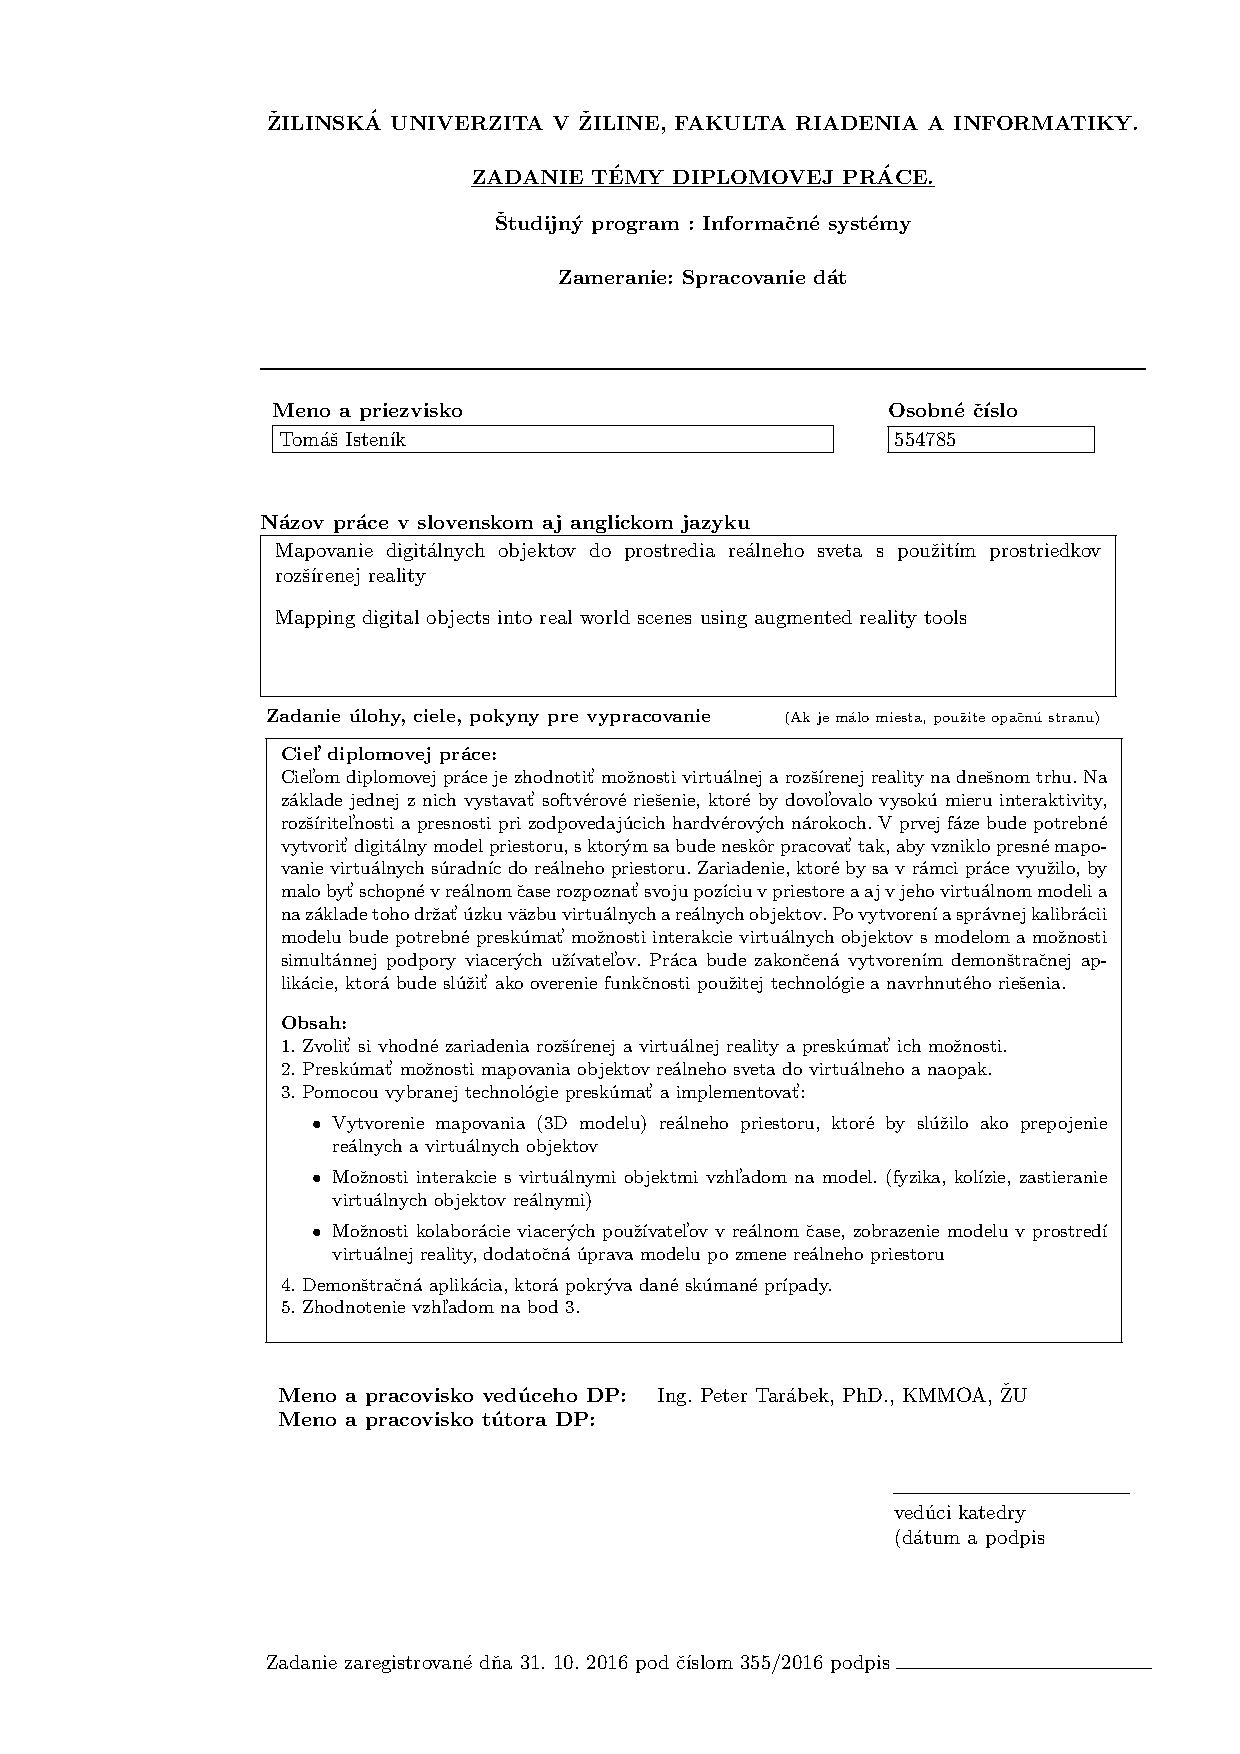
\includepdf{zadanie.pdf}

\begin{titlepage}
  
  \vspace*{\fill}
        
  \textbf{Čestné prehlásenie}\\
  Vyhlasujem, že som diplomovú prácu vypracoval samostatne, pod odborným
vedením vedúceho Ing. Petra Tarábka, PhD. a používal som len literatúru uvedenú v práci.\\ \\
V Žiline, dňa 13.4.2017
  \vspace{1.0cm}
         
\end{titlepage}

\begin{titlepage}
\section*{Abstrakt}
Práca sa venuje momentálnemu stavu trhu pre zariadenia slúžiace na sprostredkovanie virtuálnej a rozšírenej reality. Autor si zvolil za úlohu zanalyzovať súčasný stav, porovnať dostupné riešenia a pomocou vybraného implementovať systém, ktorý by umožňoval kvalitné prepojenie reálneho sveta s virtuálnymi objektami. V úvode sú popísané podmienky aj historické míľniky, ktoré ovplyvňovali vývoj zariadení virtuálnej a rozšírenej reality až po dnešný stav. Následne sú podrobne vysvetlené technické koncepty a požiadavky na rozličné systémy rozšírenej a virtuálnej reality, Po vysvetlení konceptov autor popisuje a porovnáva momentálne najznámejšie a najrozšírenejšie zariadenia a riešenia ako sú napr. Google Cardboard, Samsung GearVR, Oculus Rift a HTC Vive pre virtuálnu realitu a Epson Moverio, Google Glass, Google Tango a Microsoft HoloLens pre rozšírenú realitu. V praktickej časti autor popisuje vytvorenie troch prototypových demonštračných aplikácií, na ktorých sú skúšané koncepty ktoré overujú kvalitu skúšaných systémov alebo rozširujú ich možnosti. Prvým riešením je triviálna Android aplikácia využívajúca Vuforia AR framework na vykreslenie virtuálneho ovládača pre hračkársky RC tank. Druhým popisovaným systémom je riešenie prepojujúce Samsung GearVR a sadu interiérového ultrazvukového navigačného systému umožňujúca detekciu polohy zariadenia a pohyb po miestnosti. Tretím popisovaným riešením je aplikácia postavená nad technológiou Google Tango, ktorá sa snaží preskúmať možnosti Tango frameworku na analýzu miestnosti a vkladanie virtuálnych objektov, ktoré by boli uložené aj potom ako aplikácia stratí polohu alebo je vypnutá.\\ \\
\textbf{Kľúčové slová:} virtuálna realita, rozšírená realita, Google Tango, SLAM
\end{titlepage}

\begin{titlepage}
\section*{Abstract}
The thesis focuses on the current state of augmented and virtual reality devices market. The Author decided to analyze the market, compare the available solutions and chose a technology to implement a system allowing high-quality real and virtual objects mapping. The thesis starts with a brief look into the history and events that influenced augmented and virtual reality development in the past until the current state. After that, the bacis technological concepts for AR / VR systems are explained, as well as the requirements on such systems and the challenges they need to overcome. A deep analysis of the currently available solutions with a list of devices follows - the author adds his personal experience to the devices he had the chance to work with. The devices mentioned are Google Cardboard, Samsung GearVR, Oculus Rift, HTC VIve, Epson Moverio, Google Glass, Google Tango, Microsoft HoloLens and others. In the practical part of the thesis, the author describes creation of three prototype applications meant to evaluate or extend the possibilities of various AR / VR systems. The first prototype is a simple Android application using Vuforia framework to display virtual controls on a toy RC tank controller. The second system is a solution combining Samsung GearVR headset with an ultrasound indoor positioning system to enable position tracking for the device. The last application is based on Google Tango and it attempts to handle persisting virtual objects with their position, ensuring they can be displayed again after the application is turned off.\\ \\
\textbf{Keywords:} virtual reality, augmented reality, Google Tango, SLAM
\end{titlepage}


% table of contents
%\singlespacing
\tableofcontents

% list of figures
%\newpage
%\listoffigures

\newpage

\pagenumbering{arabic}
\setcounter{page}{8}

\specialsection{Dictionary Acronyms and Abbreviations}

\begin{definitions}
	\item[Mediated Reality] Computer-mediated reality - A summary term for adding, removing or otherwise altering one’s perception of reality with the help of computer systems such as portable computers or hand-held devices. Mediated reality serves as a wide superset of technologies like virtual reality, augmented reality or mixed reality.
	\item[MR~~~] Mixed reality - The term can be used to any system, where real and virtual objects blend to any degree, creating new environments and visualizations. The ratio in which real and virtual objects are mixed can range from almost completely real to exclusively virtual environments. Virtual and augmented realities are subsets of mixed reality.
	\item[VR~~~] Virtual Reality - A summary term for technologies and devices employing these technologies, capable of stimulating human senses in a way that creates an effect of the user experiencing a different environment instead of the real one. Generally, the most common idea of a VR device is a special headset with twin stereoscopic displays and lenses through which a user can see and interact with an artificial three-dimensional simulation.
	\item[AR~~~] Augmented Reality - A family of technologies closely related to virtual reality with the difference that instead of replacing the perception completely, augmented reality “adds” digital objects and elements into the direct or indirect view of the real world. The effect is achieved by analysing the surroundings and drawing the digital object over the real world image to create an illusion of the object actually being present. A similar, yet less known technology called diminished reality aims to remove real world objects from the screen to create an illusion of them not existing.
	\item[HMD~] Head Mounted Display - A device intended to be attached on user’s head able to display data on special displays positioned close to the user’s eyes. Depending on the type of the display and intended use, the real world image can be directly or indirectly visible to various degree or blocked out completely. One of the most important parameters of a HMD is their field of view - the parameter defining the area of human sight that the display is capable of covering with virtual objects. Also commonly regarded as a headset.
	\item[FPS~] Frames per Second - A term used for a metric defining the amount of images that are displayed on a screen during a one second interval. Higher FPS means new images are displayed on the screen more often increasing the fluidity of the image.
	\item[FOV~] Field of View - Defines the extent of the observable (both virtual and real) world that is seen or displayed at any given moment. It can be measured horizontally, vertically, or diagonally, and it defines the angular distance between the corners of visible image.
	\item[IMU~] Inertial Measurement Unit - A hardware sensor, possibly consisting of other sensors - accelerometers, magnetometers, gyroscopes etc. The purpose of the unit is to measure positional and rotational changes with maximum possible precision. An IMU plays a crucial role in most today’s augmented and virtual reality devices.
	\item[SLAM~] Simultaneous Localization and Mapping - It is a computational problem in which an unknown area is mapped by an agent while the agent is keeping track of its position within the area at the same time. Several algorithms exist today that are able to approximate SLAM calculations.

\end{definitions}

\section{Introduction}
The problematics of virtual (VR) and augmented reality (AR) has been employing technology enthusiasts from scientifical and science-fiction circles for decades, yet the technological limitations and high price generally prevented widespread commercial popularisation or restricted real world use to highly specialized areas of application. Only in recent years technologies with sufficient parameters started surfacing on the market that would offer high enough quality reproduction at a reasonable price. To fill the rapidly growing market for AR/VR has became an important goal for numerous technological giants. We are therefore witnessing new breakthroughs in the area with unparalleled frequency. While often still in development or demonstrator phases, the prototypes make their way to startups and development companies who explore their possibilities and come up with real-life problems that could benefit from augmented or virtual reality. Thanks to that, we can already experience a virtual roller coaster ride, take a walk on the ocean floor, simulate and practice in a control room of a cargo ship that has not yet been built, lay out virtual furniture in your apartment before buying it, or pilot a fast car or an airplane directly from the cockpit.

Despite the intense development in the area and unquestionable success of some AR/VR systems, numerous challenges and untackled problems remain. In order to offer high enough quality virtual reality experience, the devices require displays with extreme resolution and sufficient screen refresh rate while being able to detect headset and controller rotation and position changes precisely and swiftly enough to incorporate them into the image displayed back to the user. The result should be an user perceiving different surroundings than those he or she is physically present in. For augmented reality, the requirements are even higher - virtual objects have to be perfectly anchored to their real surroundings in various (often adverse) conditions. Overcoming these challenges often calls for custom-tailored solutions to emerge (dedicated visualization hardware, specialized sensors) but there are still many applications where AR/VR is not mature enough. 

Furthermore but also thanks to this, it is often not necessary to employ AR/VR in areas where a standard computer screen provides a more intuitive / cheaper / better solution. Finally, there are still unresolved difficulties regarding user health, especially in regard to virtual reality headsets - motion sickness, disorientation, headaches, eye fatigue etc (Not taking into account injuries or damage caused by immersing into the virtual experience too much and tripping or hitting objects in the designated VR area).

The technologies of augmented and virtual reality will have to face a long and uncertain journey before becoming an everyday part of our lives or disappearing altogether should insolvable challenges arise in the future. It is therefore exciting and favourable to be able to experience and examine the capabilities of today’s technologies and attempt to find where their boundaries are. The main questions awaiting answers are what is the current state of the AR/VR market, that level of precision do the devices offer in various price categories and what kind of problems, if any at all, are there to be solved by them.

\section{The Historical Development of AR / VR Devices}
The advent of devices and technologies, commonly known and classified as virtual and augmented reality today was preceded by a number of inventions and artistic renditions that served as predictions of future technologies and developments. From a broader point of view on AR/VR, there is a number of applications that can also meet a simplified definition of artificially altering our experience of reality. If we redefine the broader term as some kind of artificial way intended to stimulate the senses in a different than usual way, altering or enhancing the perception of reality, we might come to a conclusion that one of the simplest inventions to meet these criteria might be a simple drawing or a painting. The purpose of such picture (or any other non-abstract object for that matter) on it is to provide viewers with an idea of a country like they were present at the actual place the creation was made. One step further is a photography - analog or digital one. It generally has the same purpose of providing a view of a place, person, or an event even on a distant place or at a later time. A 360\degree~ panoramic photo brings the concept of photography into a more immersive level by capturing the whole area around of the author and letting viewers look around using their mouses or by rotating their smartphones. This results in a feeling of actually being present in the scene, yet the application is not suitable for all situation and has not replaced traditional photographs completely.
 
When looking at the current state of the art technologies, examining The Lab - a set of minigames provided for free as a technological demonstrator for a VR system HTC Vive, one of the games allows users to explore one of 4 locations in complete virtual reality and move around them to a limited extent. The locations are made in photorealistic quality and exhibit real world locations. One of which exhibits Vesper Peak, a peak in North Cascades in Washington (\nswe{48}{00}{47}N \nswe{121}{31}{04}W). The realism and immersion is so high that standing on the edge of a cliff accessible in the virtual location can induce altitude sickness and pushing the person exploring the virtual scene down can result in a panic attack.

\imgfigure{vesper_peak_vive_real}{A comparison of a real photo from Vesper Peak and its representation in HTC Vive}

Cory Ondrejka uses a similar parallel in one of his interview about Facebook and Oculus Rift involvement: a place can be described textually and the recipient then recreates a mental image of it in his or her head. A photo can be incredibly powerful, yet it only captures a single moment in time. By making a video, time is added into the experience. The last step would be the ability to capture the whole area  of a certain place and enabling the recipients to explore it in VR.

\subsection{The Pioneers of VR Concepts}
Historically, the first attempts at deliberately immersing the viewer in an artistic scene can be seen on 19th century panoramic mural paintings. The whole field of vision was filled by the picture seemingly placing spectators into a different environment.

Another key invention considered ordinary today is understanding of how human eyes work and process what they see. Each eye is able to observe single 2D sight and the process of creating a 3D model of the person’s surroundings and sensing depth based on sight is handled by the brain. The person behind this realization is English scientist and inventor Charles Wheatstone - author of stereoscope. The device uses a pair of lenses to display a stereoscopic image pair to the user creating a three-dimensional illusion. The principle of a separate screen for each eye is a cornerstone of today’s VR and AR devices.

\imgfigure{stereoscope_cardboard}{A classical stereoscope shares a lot with today's Google Cardboard VR headset.}

As the world advanced, the technological progress in many areas allowed for a wider area of utilization and practical applications became more frequent. One of the first industries to start benefiting from virtual experience creating a simulation of reality was aeronautics and military. Edwin Albert Link, an American aviation and underwater archaeology pioneer created a device known as “Blue Box” or “Link Trainer” that is today considered to be the first flight simulator ever created. The electromechanical device was used in basic pilot training to promote faster, cheaper, and safer ways to obtain skillful pilots. The device could mimic responses to flight controls and and gave an accurate reading on cockpit instruments, helping the trainees learn utilize them when piloting. During WW2, more than 500,000 American  pilots had a part of their training done on a Blue Box.

\imgfigure[h][\textwidth/4]{link_trainer}{Link trainer was a device that roughly simulated real airplane behaviour to let pilots train in safer and cheaper conditions.}

Along with technological development, we can also look back on historical cultural predictions in the form of science-fiction literature and movies that undisputedly helped shape the world we live in today. It was already in 19th century Jules Verne predicted inventions like submarines, television newscasts, videoconferences or human landing on the Moon. A work of fiction strikingly similar to today’s augmented and virtual reality headsets came from the pen of  Stanley G. Weinbaum in 1935. The short story - Pigmalion’s Spectacles elaborates on an idea of a pair of goggles allowing their user to experience a fictional world via holographics, sound, smell, taste, and touch. The googles also allow the user to interact with the world - it is possible to talk to fictional characters named shadows with them being able to reply back. In 1901, American Author L. Frank Baum released The Master Key - a novel about a young boy who is given a set of magical artifacts from a supernatural “Demon of Electricity”. Amongst these is a set of spectacles that place a letter on the forehead of anyone the wearer sees depending on their personality and traits.

\subsection{1960s - The First Virtual and Augmented Reality Devices Appear}
Since the technological concepts have already been defined and the age of microchips steadily seeped into everyday life, the first practical attempts started emerging, along with more concepts being defined. During this period, up until around 1990, most if not all VR concepts have been lain out and the only technological challenge has been to increase the image replication quality. Augmented Reality is generally more complex, having to juxtapose virtual reality with area learning and real objects detection.

In 1962, Morton Heilig, a pioneer in VR technology and a cinematographer patented his multi-sensory, immersive cinematic machine called Sensorama, built 5 years earlier. The prototype machine served as a vision of the future of cinema, where multiple senses would be stimulated and the viewers would be engaged further. The arcade-style theatre cabinet device contained stereo speakers, a stereoscopic video display, fans, smell generators and a vibrating chair. The short films that could be played on the device were named Motorcycle, Dune Buggy, Belly Dancer, Helicopter, A Date with Sabina and I’m a Coca Cola Bottle.

\imgfigure[h][\textwidth/2]{sensorama}{Sensorama attempted to predict the cinema of the future that would stimulate as many senses as possible.}

Another invention from Heilig, the Telesphere Mask, patented in 1960, is considered the first ever HMD, despite not supporting any interactivity or head position or movement tracking. The device offered a pair of stereoscopic widescreen displays as well as a pair of stereo speakers. Another head-mounted display, this time with simple head tracking, called Headsight, was developed a year later. Its authors, Comeau \& Bryan from Philco Corporation used a magnetic system to determine rotation of the headset and a single CRT element for displaying. The intended purpose of the gadget was to provide remote sight in dangerous situations using a closed circuit camera.

In 1965, Ivan Sutherland, an American computer specialist and internet pioneer, widely regarded as the “father of computer graphics”, laid down a document that would later become a core blueprint for concepts encompassing virtual and augmented reality today. Named “The Ultimate Display”, the paper investigates the ways in which computer data could be displayed to the users as well as what approaches are there to input data into computers. Ultimately, he describes systems that would monitor the movement of each human muscle or eye focus and generate and maintain entire simulated virtual worlds as realistic and tactile as reality.

\begin{displayquote}
\textit{“The ultimate display would, of course, be a room within which the computer can control the existence of matter. A chair displayed in such a room would be good enough to sit in. Handcuffs displayed in such a room would be confining, and a bullet displayed in such a room would be fatal. With appropriate programming such a display could literally be the Wonderland into which Alice walked.“}
\end{displayquote}
\begin{flushright}
- Ivan Sutherland
\end{flushright}

In 1968, together with his student Bob Sproull, he created the first ever augmented and virtual reality head-mounted display system called The Sword of Damocles. Its technological primacy lied in the fact that it used a computer generated image for the display instead of using cameras like former systems, as well as in the fact that the image shown to the user depended on where he or she gazed - calculating the direction in which the user is pointed is called head tracking. The Sword of Damocles name originated from the fact that the headset was suspended from the ceiling on a mechanical arm and securely fastened to user’s head. The components of the system were not fully interconnected and the whole contraption’s main purpose was to serve as a prototype for “the ultimate display” research. The display showed primitive wireframes (limited by the computing power of general-purpose computers of the time) with the unit being partially see-through. Thanks to that it is today considered to be one of the first augmented reality precursors.

\imgfigure{damocles}{Sword of Damocles HMD was named after its intricate appearence. The device was capable of rotational tracking.}

Another of the milestones towards today’s AR / VR as we know them was the work of Myron W. Krueger, an American computer artist accountable for many early interactive works and considered one of the first virtual and augmented reality researchers. He is behind a series of gradually improved interactive experiences called GLOWFLOW, METAPLAY, and PSYCHIC SPACE which ultimately progressed into a technology called VIDEOPLACE. The idea of the technology was to immerse users in a virtual experience without the need for any goggles, gloves or other wearable hardware. Instead, a set of projectors, cameras, on-screen projections and specialized hardware surrounded the users and responded to their movements and actions. To interact with others, a silhouette was created from the person and projected on the wall as an avatar where it could interact with other users also represented as silhouettes. Kreuger summarised his experience in the area of interactive artificial worlds along with his future visions in his 1983 book Artificial Reality and its revised version Artificial Reality 2 in 1991.

Back in 1978 at MIT, a revolutionary hypermedia system was developed by a team led by Andrew Lippman with fundings from ARPA (Advanced Research Projects Agency). Called Aspen Movie Map, it was the first predecessor of systems like today’s Google Street View. The original motivation behind the system was enabling soldiers to familiarize with unknown environments quickly and was inspired by Israeli commandos’ Operation Entebble in 1976, where the soldiers built a crude replica of an airport terminal to train before commencing the real operation. Aspen Movie Map was a system providing virtual tours of the city of Aspen, Colorado. The researchers used a car with 4 orthogonal cameras to create a view of the city from a travelling car every 3 metres. The interactive system was touchscreen controlled and it allowed the user to create a travelling path in a city-map view and then enjoy a surrogate car ride among the specified path. Three modes were available: early autumn, winter, and computer generated wireframe and could be switched at any time.

In 1980, Canadian researcher and inventor Steve Mann created one of the first wearable computers. The system combined a computer vision system with graphical overlays on photographically mediated reality and could basically allow the human eye to serve both as a camera and a monitor. The mechanism was placed directly in front of a human eye and it records the view using a lens, processes it and displays it back to the eye using the same lens, possibly being augmented with digital data. Called “Digital Eye Glass”, “Eye Glass” or “Glass Eye” by its inventor, the heavy and cumbersome device covering the whole head ultimately evolved into EyeTap, which, while using the same principle looks like a fairly ordinary eyeglass frame. One of the main advantages of the design is the image perceived by the camera is exactly the same as the one seen by the eye so mapping digital objects using computer vision and image processing has great potential in terms of augmented reality (the original image and the real surroundings are still visible to the user). EyeTap, in terms of its appearance and capabilities, can be considered to be the 10 years older brother of Google Glass. Mann predicts that in the near future most people will use wearable headsets with camera capabilities enabling us to record every moment of our lives (This is a questionable claim for the near future considering Google Glass did not hit mainstream success).

\imgfigure[h][\textwidth/4]{steve_mann}{Mann with his 1999 Eye Tap prototype that looks remarkably similar to Google Glass.}

\subsection{1980s - Virtual Reality Comes to Life}
The term \textbf{Virtual Reality} that is generally widespread today was actually popularized by Jaron Lanier, an American computer scientist, visual artist, and a music composer through the second half of 1980s. His company, VPL Research, founded in 1984, was among the first companies to develop and sell virtual reality devices commercially. Lanier originally worked for Atari Inc in their dedicated virtual reality lab, but after the North American video game crash of 1983 the lab got closed down and Lanier along with his colleagues became unemployed. VPL Research brought several VR devices to the market: Data Glove - an input system tracking hand movements and orientation, EyePhone - a HMD with fresnel lenses and head movement tracking capabilities, Data Suit - a full-body outfit capable of tracking and measuring movement of trunk and limbs. Despite initial success the company filed for bankruptcy in 1990 and the remaining patents were bought by Sun Microsystems in 1999.

Long before virtual and augmented reality hardware even started becoming widely accessible for household ownership, some degree of public exposure was provided when Virtuality Group (originally named W Industries), a United Kingdom based company started offering a range of arcade games and machines. Players enjoying this experience would use 3D head mounted displays and various joysticks, steering wheels or aircraft yokes (depending on the system and game) for controls. Some systems supported multiplayer by having several stations networked together. Their headset tracking real-time response was only 50 ms (today, 16 ms is considered to be the limit). Two device types were available depending of how the player was positioned: sitting and standing units. The display resolution was 276x372 pixels for each eye and apart from the stereoscopic LCD displays, each headset contained 4 speakers and a microphone. A magnetic system was used to detect head and controller movements and allowed the system to respond accordingly. Despite being initially a huge success and stating its aim to be far beyond simple entertainment systems, Virtuality Group failed to deliver convincing advancements and filed for bankruptcy in 1997.

\imgfigure{virtuality}{Virtuality was arguably the most successful VR company in the 1990s.}

One of the milestones undoubtedly interconnected with the rapid rise of virtual reality in the early nineties was The Lawnmower Man directed by Brett Leonard in 1992. In the sci-fi action horror movie, a scientist uses a mix of intelligence enhancing drugs and virtual reality on a simple-minded gardener to improve his cognitive abilities. After some time the experiment spirals out of control as the test subject is able to take control and start pursuing his own goals. The movie was strongly inspired by Jaron Lanier, VPL, and other VR companies of the time. This is easily visible in the fact that many of the props used thorough the movie are actual VPL equipment and the opening credits of the movie predict VR to be in widespread use by 2000 with all possible positives and drawbacks the technology could bring humanity.

Not much longer after arcade machines from Virtuality initially succeeded commercially and marked a new potential market, major home entertainment system manufacturers announced their own virtual reality systems. Sega announced its Sega VR headset in 1993. Coupled with a Sega Genesis or Saturn console, the headset would have twin LCD display and stereophonic speakers. Inertial sensors would allow the headset to respond to head movements. Complications during development and possible problems with headaches and motion sickness prevented the console from ever reaching beyond prototype stages. A similarly grim fate awaited a competitor product, Nintendo’s Virtual Boy. It was supposed to be the first portable console with 3D graphics and was actually commercially released in Japan and North America, but its specifications were nowhere near desirable. The portability of the console was questionable, it was uncomfortable to use, only offered a red and black display and most of the games did not benefit from being 3D at all. No head movement tracking was supported.

Between 1995 and 2000, the market of AR and VR devices started to fall as the expectations from the technology were displaced by the overwhelming technical limitations of computer electronics of the time. During the nineties, AR and VR was seen as the next technological step in technological development and much energy was invested into making higher precision devices possible. There are two main reasons for the hype dying out as the new millennium approached. The hardware was remotely not powerful enough to enable precision and interaction levels beyond basic graphics thus limiting the potential usages to very specific cases also negatively affecting the market potential. Secondly, the main focus of most companies switched to the internet as it became the most anticipated and promising technology at that time, leaving AR and VR behind for some time. This does, however not mean the development stopped completely - many companies remained operative, often thanks to specific field contracts like military simulation or universities, but the general public stopped being so interested in the technologies until acceptable quality devices become widely available.

Perhaps the most influential movie where virtual reality as a concept played the main role is 1999’s The Matrix by The Wachowski Brothers. In the movie a computer hacker is contacted by a group of rebels to learn that he’s been living his entire life in an extremely realistic computer simulation. There are no HMDs or other kinds of hardware used, the connection into the simulated world can be done directly via a brain interface basically breaking all bonds between user’s body and mind. The movie has both envisioned a possible peak of both virtual reality and computer system user interfaces (by having a brain-computer interface directly on the body eliminating the need for displays and input peripherals) and restarted a debate about the possible consequences of such technologies.

A little less technologically advanced form of virtual reality, very close to Ivan Sutherland’s Ultimate Display appeared in Star Trek: The Next Generation. Nicknamed the Holodeck, the system is capable of simulating matter together with complete interaction and even being possibly harmful to its users. Holodeck itself is a room of considerable proportions within which the virtual phenomena was simulated.

\imgfigure{holodeck}{The sci-fi simulation room - Holodeck, where everything can be adjusted by the computer, fits to the vision of Sutherland's Ultimate Display.}

\subsection{2000s - The Development Continues}
After the wild blossom of AR/VR technologies in the nineties and despite the virtual reality hype dying out, a wide range of companies and universities continued pushing the boundaries further and finding new areas where the concepts could be employed. In 1999, Hirokazu Kato released the first version of ARToolKit, an (now) open source library for augmented reality using special trackers - tags / ARTags. The library is still being developed and  remains one of the dozens readily available AR/VR solutions on the market. From 1999 onwards, several augmented reality technologies were tested that overlaid virtual map data over real world video simplifying navigation and awareness. Similar programs gradually emerged for military use. The development was continuous and the technologies slowly creeped into more and more areas - medical, entertainment, navigation, translation etc. The first cubic room, SAS3 or SAS Cube was created in 2001 in France by Z-A Production. This type of a VR system is today widely regarded to as CAVE (cave automatic virtual environment). It usually consists of a cubic room combining a set of projectors on three to six walls and other specialized hardware intended to help viewing (3D glasses) or interacting with the virtual simulation.

In 2007, 29 years after Aspen Movie Map, Google launched Street View, a technology featured in Google Maps and Google Earth that enables panoramic views of city streets for select American cities. The technology has since expanded to contain practically every city in the world letting anyone with internet connection to virtually travel to any destination. Together with online maps and GPS navigation, it is today easily possible to explore a place before physically visiting it, allowing us to check a hotel’s surroundings or road directions before even deciding to travel there.

In 2011, the first prototypes that eventually gave birth to Oculus Rift was made by Palmer Luckey, an American entrepreneur who eventually founded Oculus VR company to enable commercial use of his devices. The project later sparked a Kickstarter campaign and basically started what can be considered the second VR revolution today. Luckey originally developed several prototypes with various parameters, sizes and weights. His first prototype, built into a different headset’s body, only supported rotational tracking, but it incorporated 90\degree~ field of view, previously unseen on the consumer market. The HMD also inspired Id Software to announce 3D headset support for their Doom 3 release.

The situation was not so bright in the augmented reality sector. The technological difficulties encountered in AR devices are often more complex than those in VR and there are usually tighter constraints regarding the device’s raw computational power. LyteShot, an augmented reality gaming platform by a same-name company, launched in 2012. Using specialized hardware and smartphones with bluetooth connectivity, the devices enable various types of real-life games with digital processing handling things such as scoring, game quests, removing players from the game etc. Today, similar systems are widely used in laser-tag arenas, where players can see their scores and real-time metrics instantaneously. Meta, a Silicon Valley based company, launched a Kickstarter campaign for what would later become one of the first see-through augmented reality glasses - Meta 1 development kit. The company was aiming to provide a means of displaying virtual objects in real world for uses like medical training or engineering. The headset boasts twin displays, accelerometer, gyroscope, compass, and a depth perceiving camera. Field of view is limited to 23\degree~ per display and the headset weighs 300 grams.

One of the most influential and publically known augmented reality devices was Google’s Google Glass which was announced in 2012 and entered public beta in 2013. The first internal prototype of the device using a head-mounted display weighed over 3 kilograms. The publically available version of the device is lighter than a pair of sunglasses. The computational power is somewhat limited and most of the resource-heavy calculations are done on a smartphone, to which the glass is paired via bluetooth. Hardware-wise, Google Glass has a 720p camera, bone-transmitting audio conductor, a microphone, 640 x 360 LCoS (liquid crystal on silicon) display using a collimating reflector to direct the beams into the wearer’s eye, 1 GiB of RAM, dual-core 1,2Ghz ARM CPU and 12GB of memory available to the user. Interaction with the device was possible via an intuitive touch panel, voice commands or even head movement gestures. Movement was tracked by a 3 axis gyroscope, 3 axis accelerometer and a 3 axis magnetometer (compass). Google announced that Glass would be discontinued in 2015, stating that its development will continue until commercial-readiness is achieved.

Design-wise, Google Glass is meant to work as a supplement to a smartphone, simplifying and extending its use. Taking photos or videos does not require using one’s hands and various notifications such as SMS messages or social media mentions get displayed to the user directly. The short battery life together with high price and scarcity of useful applications would be the main reasons for discontinuing the wearable. Some degree of use was found nevertheless - healthcare, journalism and military all benefitted from the hands-free interface and the portability of the device’s camera. However, both the SDK support and computational power do not provide nearly enough functionality to support more sophisticated AR applications.
https://developers.google.com/glass/distribute/glass-at-work

\subsection{Current Technologies}
One of important breakthroughs in VR display technologies was made in 2013 by Valve Corporation in the field of display persistence. In order to ensure nausea-free and highest-possible quality immersion, the screen must be refreshed as often as possible without any interruptions. Sixty \textbf{frames per second} (fps) is considered the absolute minimum for believable virtual reality experience, although it is believed, refresh rates as high as 1,000 Hz are needed for a perfect experience - something we can not achieve with current technology. The breakthrough, so important for VR was a new type of display with considerably lower persistence rate, which, together with using strobing/black frame periods allowed for lower motion blur effects and sharper display. All subsequent VR headsets employed this type of displays.

Another development that turned out to serve as a basis for two of today’s best VR headsets was Valve’s internal Steam Sight prototype. The technologies for the headset itself (not positional tracking) ended up basically unchanged in production versions of both HTC Vive and its concurrent Oculus Rift HMDs. Value claims to have lent a single Steam Sight piece to Oculus VR before it was acquisited by Facebook in 2014 with Oculus using it as an inspiration while working on Rift.

A device meant to encourage VR awareness and developer interest in the technology, named Google Cardboard was announced on Google I/O conference in 2014. The Cardboard belongs to the lowest price category for VR devices and is meant to be coupled with a smartphone - thanks to that, the cost of a single unit is only around 15\$. It basically consists of a primitive cardboard headset with 2 lenses and a magnetic button used to interact with the device (phone’s internal compass is used to detect interaction). Motion (rotational) detection relies on the phone’s accelerometers and gyroscopes. A great amount of similar HMDs have since been created and are available on the market with Samsung’s GearVR possibly being the best known one.

Apart from Oculus, which gained a massive momentum boost in 2014, when it was acquired by Facebook for over 2 billion dollars and is shipping the consumer version of Rift today, two more virtual reality headsets hold a strong position on the market, Playstation VR by Sony, originally codenamed Project Morpheus, first announced in 2014 and HTC Vive, a cooperation between HTC and Valve. All three headsets support full positional tracking and various kinds of controllers are supported. Rift was released in April 2016, Vive one month later, Playstation VR came out in October 2016.

\imgfigure{htc_oculus_psvr}{The best three VR headsets currently available - Vive, Rift, and Playstation VR.}

An interesting technology with considerable AR potential that has recently reached consumer availability is Google’s Tango, previously known as Project Tango. Originally announced in 2014, the AR platform combines computer vision, depth perception, and motion tracking to provide high quality information about the surroundings the device is in. Thanks to the technology, a tango-enabled device is able to create 3D models of rooms and objects, measure distances inside rooms or ad virtual objects into real world. Currently, one Android smartphone supports the technology - Lenovo Phab 2 PRO, with Asus announcing its Tango phone - ZenFone AR in January 2017.

The current state-of-the-art AR technology is currently believed to be Microsoft’s HoloLens. Currently available worldwide as a developer edition and originally introduced in January 2015, its roots can be traced back to 2010, when Kinect - an add-on to Microsoft’s Xbox gaming console, was released. HoloLens is a headworn HMD with twin see-through displays and hi-performance hardware that is capable of placing virtual holograms into the user’s surroundings and track their positions there. There are a number of features that appoint HoloLens the best AR platform currently available with only a few possible drawbacks: price (3000\$), field of view (estimated to be 30\degree~x 17.5\degree~ for each display), and battery life of 2 to 3 hours. 

\imgfigure[h][\textwidth/4]{hololens}{With gesture controls and massive performance considering it's a mobile device, HoloLens currently offers the best AR experience on the market.}

As of early 2017, there are hundreds of companies working on AR and VR applications in a wide area of applications both applying the current technologies to real life and extending the possibilities with new technologies. With the arrival of Oculus Rift, HTC Vive, and Playstation VR, more and more customers are engaged into virtual experiences in their homes or trying them out in businesses that rent them. Similarly, the AR market saw considerable public exposure with Niantic’s Pokemon GO mobile game, that was released for Android and iOS in July 2016 and saw massive success. The player’s position in the game world depends on his or her real life position using GPS and once catching a virtual companion in the game, the pokemon would be displayed in the real world using phone’s camera. Google’s continued expansion into the VR market led to Google Daydream, a cardboard-like headset meant to be used with a daydream-ready phone. The headset does have a special controller with gyroscope and trackpad that is arguably more comfortable to use than Samsung’s GearVR that has a gamepad on its right side. In March 2017, Apple Inc’s CEO TIm Cook has announced the company will focus on AR market development in the short future, seemingly confirming the fact that the market is going to see even greater expansion in the upcoming years.

\section{Technical Specifications and Requirements}
Depending on the technology used and the overall design of various systems, a diverse amount of advantages and drawbacks can be identified for every system. This chapter explains the requirements that need to be met in order to offer the highest quality object mapping and experience. 

There are two main objectives to be handled by the AR and VR systems: position and environment detection and displaying virtual objects. The first system is responsible for figuring out the position and alignment of the device, passing these parameters to the engine and renderer, ensuring the image displayed to the user aligns with positional and rotational changes perfectly.

\subsection{Basic Concepts}
\subsubsection{Headset Position Detection}
For the clarity of the explanation, we will consider any device meant to display virtual or augmented experience to be a headset. Basically, there are two types of devices in this category - screens (computer, handheld device) and actual headsets (single eye, full-face HMDs). In order to make the headset appear in virtual space closely tied to reality, all its movements and translations in the real world should closely correspond to changes in the virtual world display. Here, the term \textbf{six degrees of freedom} (6DoF) is most commonly used. The term relates to three possible translation and three rotation axes, specifically translation forward/backward, left/right, up/down and rotation about three perpendicular axes - pitch, yaw and roll. Not all headsets support every axis movement/rotation detection, though they are all necessary for augmented reality applications.

The most trivial to solve are the three rotation axes - a headset with precise accelerometer, gyroscope and magnetoscope can quite successfully approximate its orientation and acceleration (accelerometer data), rotation changes (gyroscope) and current heading (magnetometer or compass). These internal sensors are present in most smartphones today making Google cardboard-based VR easily accessible, though moving one’s head does not get translated into the virtual world. Another drawback of this system is the relativity of heading. Usually, the virtual world will be displayed in the heading the user puts the headset on.

For the position axes, specialized systems need to be utilized - from external sensors detecting headset position to depth cameras and computer vision scanning the device’s surroundings. Generally they vary with the area they can cover, their position, precision and price.

\imgfigure[h][\textwidth/4]{6dof}{Six degrees of freedom illustrated - three translation axes and three rotation axes exist.}

\subsubsection{Displaying Virtual Objects}
In order to render objects in virtual space, a camera has to be specified with a position, orientation and other parameters such as field of view, to know what objects will be displayed in the final image. Most 3D rendering software today works without augmented and virtual reality position detection, only changing the position based on user input from keyboards, mice, joysticks or other devices. The subtle change done by mixed reality systems is relying on position detection systems for this input. For handheld devices such as phones with augmented reality-enabled applications (most often using device cameras) or Google’s Project Tango-enabled phones, the requirements are basically the same as for any other 3D program - some amount of lag, delay, or drift is acceptable, yet undesirable. On the other hand, HMDs need to tie the rendered objects with real-world device orientation perfectly with the lowest-possible delay, making them significantly more performance demanding. There generally need to be two stereographic images instead of one, they require special lens distortion - a counterreaction to physical lens distortion, ensuring wide field of view, and 60 frames per second at all times is the bare minimum to minimize motion sickness. There are several approaches to solve these problems based on the requirements and technologies used.

\subsubsection{Virtual Reality Sickness} 
The main reason for such a gap in the requirements placed on handheld and on-screen mixed reality devices and HMD-based systems lies in the way they affect perception. When external screens are used, users easily recognise that the image on the screens is emulated and despite being closely tied to real world, not replacing reality in any way. With HMDs, especially virtual ones, real world perception is dampened and users have to completely rely on the virtual experience. The human body uses two main mechanisms to orient itself in space: visual orientation and the vestibular system. The first consists of understanding the shape of our surroundings and positioning and moving ourselves accordingly. The latter is a sensory mechanism located in the inner ear, capable of detecting translation and rotation changes\footnote{A test popular amongst children that proves the systems work together is to try standing on one leg while keeping balance with and without one's eyes closed.}. If the stimuli coming from both systems does not match up (eg. movement in the virtual environment while not feeling any inertia) or are of inconsistent quality (lag, latency spikes, high persistence displays, motion blur), sickness and discomfort may appear. There are many potential factors affecting virtual reality sickness and the whole area is not yet fully understood.

For augmented reality headsets, the virtual reality sickness does not pose a problem since real-world perception is still present, but high-performance detection is still desirable to ensure virtual objects do not twitch and are solidly anchored to their real space coordinates.

\subsection{AR / VR Device Classification}
In order to be able to compare the technologies and their capabilities, it is essential to identify which parameters play a crucial role defining the strengths and drawbacks of each platform. The possible ways a device could be utilized depend on factors like price, availability, portability, quality of movement detection, detection area limitations, computational power, support, development tools quality etc.

\begin{definitions}
\item[Price] Defines the availability of the product plus a soft constraint on the performance. Currently, the cheapest ways to get to both AR and VR can start at 0 - 50\euro, provided a smartphone, tablet or a computer with a camera are present. A device with a camera can learn to recognise special markers and add a virtual object into the camera screen thanks to one of the numerous AR frameworks available today. In the VR market, a headset is required - Google Cardboard is the cheapest way of converting a smartphone into a simple headset. More expensive smartphone mounts exist up to Samsung GearVR, which retails for about 130\euro~ and only works with Samsung Galaxy S6 and S7 models. In the mid-range, devices like Playstation VR, Oculus Rift, HTC Vive for VR and Lenovo Phab 2 PRO, Epson Moverio etc. for AR offer reasonable experience (provided other hardware is already present for PSVR, Rift, and Vive to run on) in the 400 - 1,000\euro~ price range. Further down the line, now discontinued Google Glass explorer edition originally retailed for \$1,500, Microsoft HoloLens developer preview version is available for \$3,000. Specialized filmmaking motion tracking environments and CAVE systems can cost up to hundreds of thousands euros while offering flawless precision.

It is important to consider additional costs of a system when examining the total price - powerful smartphones are needed for cardboard-type headsets, Vive and Rift require VR-ready computers, Playstation VR needs the PS4 console etc.
\item[Performance]A combination of the computational power and the quality of virtual object rendition. A more powerful device is generally able to display more complex sceneries at a lower delay and higher refresh rate and precision. Generally, the final screen gets rendered as a compromise between scene quality and rendering speed and high-complexity calculations should be avoided to leave out enough capacity for position detection arithmetics. Microsoft Hololens even employs a specifically designed hardware chip, called holographic processing unit (HPU), that solves this problem by performing position detection calculations.

There is generally a noticeable performance gap between mobile-device based AR/VR systems and those that employ dedicated computers.
\item[System topology] Closely related to the technologies used by the platforms - it defines how what are the standalone parts of the system and how they interact with other in relation to their role and physical position. An ideal device would consist of the headset / display unit only with no other auxiliary hardware. This is, however, currently impossible and a number of systems uses external peripherals to help solve some of the technological challenges. The sensors that detect device movement / orientation can be mounted in the room externally (with the room being calibrated before the AR / VR platform is used) and the HMD is often connected to a high-performance computer via a cable. This lowers the weight of the HMD, eliminates the need for a battery and provides higher computing power and precision, but limits both the user and the area physically.
\item[Portability] Heavily depends on the topology of the system. Generally, the more parts are present, the harder it is to use the system in a new area, but there can be further problems like light conditions interfering with the systems or high calibration demands. Systems which rely on external power sources cannot be used anywhere.
\item[Position detection type] As mentioned earlier, not all six degrees of freedom are supported on all devices. The simplest VR solutions such as a 3D video played using a Cardboard, do not support any translation or rotation axis detection. Phones compatible with Cardboard-type headsets are able to support rotation - roll, pitch and yaw. There are also devices capable of presenting location, but not orientation - indoor positioning systems employing diverse technologies such as ultrasound, bluetooth, or wifi with varying levels of precision - mostly insufficient for AR/VR use. Apart from the basic detection performance metrics, there are further possible constraints and prerequisites linked with the technologies used. Some systems only detect position if their sensor stations have direct visibility to each other or the user is facing a certain direction. For some systems, it might also be problematic to add more than one headset into the area. Currently, most AR/VR systems on the market use accelerometers, gyroscopes, and magnetometers for rotation detection along with cameras and image recognition, depth cameras, and IR-sensitive detectors to calculate both position and rotation changes. The ability of systems to detect precise absolute rotation is also not present in all systems - in those cases, the heading that an user starts with after putting on the headset defines virtual space orientation.

The important metrics for position detection are: position detection precision (how precisely is the headset’s position detected, also affects the tendency to “twitch”), frequency (how often does the system generate a new position measurement), delay (how current the measurement is - the time period between measurement and its availability to in the device). For rotation detection, the ability of the system to know absolute rotation plays a role.
\item[Supported area size] Relevant for devices that support movement through virtual space. It may vary from a small space limited to head movement only through a rectangular room up to 5x5 metres to a virtually unlimited space for devices not requiring sensors or manual room calibration. There are two main reasons for limiting the active area: the technology used might be constrained (external sensors, camera field of view, headset cable length) and the intended use of the system might call for a limited area size (virtual plane cockpits, virtual game areas).

\imgfigure{vive_area}{An illustration of how Vive Lighthouses can cover up to 5 x 5 m area. The boxes do not require any synchronisation with the computer and only need electricity connected.}

\item[Controller support] Ways to interact with the virtual objects are essential to advance the experience beyond simple observation. These can be as simple as a set of buttons on the side of the headset or GUI elements on the screen (for augmented reality phones). It is also generally possible to use various external gamepads, joysticks or steering wheels, but these peripherals have a visibility drawback - people using virtual reality headsets are unable to see their hands or other surroundings including the controllers. For this very reason dedicated VR systems use specialized controllers capable of being tracked in virtual space, that users can see. Microsoft HoloLens uses 3D cameras to recognise hand gestures, eliminating the need for an external controller completely (pointing is done by rotating one’s head).
\end{definitions}

\subsection{Display Characteristics}
Superb display properties are one of the crucial concerns for virtual reality headsets and highly important for augmented reality goggles. One of the keys to high immersion and sickness-eliminating experience is fluid image with high frame rate, low persistence and motion blur, high (ideally 4k) resolution with an invisible mesh (area between individual pixels). Additionally, field of view matching that of human the eyes for all types of displays would be ideal to provide flawless experience. Augmented reality headsets employ see-through displays with collimated light that projects the virtual objects with a distant focus, virtual reality collimate light with fresnel lenses.

\begin{definitions}
\item[Resolution] Defines the summary amount of pixels in both horizontal and vertical dimensions. As per most computer performance metrics, higher is better, especially since the screens of head-mounted displays are located very closely to user’s eyes and higher resolution allows for sharper and more detailed image. There are however massive drawbacks to increasing the resolution - there are two displays in a headset, each with its own image. Thanks to the fact that the frame rate has to keep high at all times, various optimisations and sacrifices are often employed with screen resolution possibly being one of them.
\item[Density] The resolution of a screen is not the only parameter defining its physical appearance - different size displays can have the same resolutions if a single point’s size on each is in the same proportion to the size of the display itself. Density defines physical size of pixels on a display, or, more precisely, the amount of pixels present per a single unit of area. Pixels per inch (ppi) are used most often. The reason screen density is important in virtual reality headsets is the maximum resolution a human eye is able to perceive - 0.3 arcminutes per pixel. If we wanted to create a screen with resolution corresponding to human eye that would occupy 90 by 90 degrees (which is considerably less than the eye can really see), the required resolution would be at least 18,000 by 18,000 pixels - something that is impossible with today’s technology, especially considering other important display metrics. Furthermore, the eye does not work as a display and can rotate around, changing focus freely, while the display remains stationary.
\item[Frame rate] Means the frequency the image gets updated on the display. The absolute minimum for virtual reality is 60 frames per second, though this is not enough if we also consider screen persistence and delay. The industry standard for motion picture and computer applications has long been considered to be 24-30 fps, but recently, manufacturers started switching to 60fps, which is more smooth and fluid especially in dynamic scenes. Since in VR the user’s visual sense of stability depends on the image from the headset, the image needs to be redrawn as often as possible with the newest position information, or the risk of virtual reality sickness-related problems increases. There are several possible issues that might affect frame rate negatively: lag spikes or frame skips, where the rendering is paused for a time period, can cause the image to freeze during head movement, degrading the experience. It has been proven that constant lower frame rate is perceived better, than high frame rate with noticeable lag spikes. Another possible problem, not directly related to frame rate, is image delay - the time period between physical user interaction (moving one’s head) and it being reflected in the virtual world - ideally, no image delay should be present.

Various researches suggest the human eye is able to react to stimuli at up to 1000 fps speed, so it is probably safe to assume the ideal experience will not be achieved in the following years and alternative ways to simulate high frame rate are needed.
\item[Persistence] The metric defining how long the image stays on the screen after being drawn. Lowering it is one of the ways to mimic higher frame rates and reduce VR sickness and motion blur. With 60 fps video and full persistence, each frame stays on the screen for 16.6 ms. This basically means the image remains still for the whole duration of the frame. The consequences are mostly negative - if the head position is changing over time, the virtual image will does not reflect it until a next frame gets drawn 16 milliseconds later. The resulting judder creates the illusion that the environment is moving together with the headset and resets itself to its initial position repeatedly. If the distance of a single point changed more than several pixels between frames, a motion blur effect happens which degrades the experience severally. A method how to work around this problem, although not without its own drawbacks, is to lower the time the image stays on and show black during the remainder of the frame. This method increases the sharpness and fluidness unless the movement is too fast, when the frames become drawn too far apart. This effect, where multiple images can be perceived instead a single dynamic one is called strobing.
\item[Display mesh] The size and visibility of the area in between actual pixels. It is closely related to the display resolution and ideally it would be not noticeable. It was speculated that together with lower-than-optimal resolution of today’s VR headsets, would not provide enough sharpness to make the applications useful, as the mesh would obstruct view to details of the virtual environment. This is only partially true - by moving one’s head, the eyes can easily fill in the missing pieces of the image and the mesh does not disturb users severely. It is, however, still worth noting that in systems that support both VR and standard screens, the difference in sharpness is easily noticeable in favour of classical computer screens.
\item[Field of view] Defines the extent of the observable (both virtual and real) world that is seen or displayed at any given moment. It can be measured horizontally, vertically, or diagonally, and it defines the angular distance between the corners of visible image. The term used to define the corresponding term for humans and animals is visual field. Both virtual and augmented reality headsets cover a certain percentage of human sight with displays while the uncovered area is either obstructed or unchanged by the device. For non-headset devices, field of view depends on their camera’s properties and display settings (in case the image is cropped). The general aim for mixed reality systems is to cover the whole eyesight in both horizontal and vertical dimensions. Currently, virtual reality headsets are capable of rather impressive and sufficient angles, but augmented reality systems often suffer from small screen sizes, usually limiting their FoVs to well below 45 degrees.
\end{definitions}

\imgfigure{fov}{Field of View illustrated. A screen that is closer to the eye needs higher density to retain image quality. A head mounted display is an extreme case.}

\subsection{Development Support}
In order to reach its full potential, it is crucial each technology exposes a set of development tools to allow application developers employ it for new solutions and applications. There is a positive feedback loop between the amount of application available for a technology and its popularity - the more applications were created for a platform, the more popular it becomes, increasing its market and user base and attracting new developers in. From this point of view, it is desirable to simplify content creation by providing software development kits for popular already-existent frameworks. Generally, there are several frameworks present for each technology, varying in the programming language level they work with. Thanks to this, applications utilizing the technologies can choose the level of performance to development time tradeoff that is sufficient for them. This enables both precision and performance-heavy applications as well as rapid prototyping examples to be created with reasonable schedules and resources.

Most mixed reality solutions today provide frameworks for programming applications in C++, java or similar, where only the basic functions relevant to the specific framework API are exposed and it’s up to the developer to employ them to get the final product, and higher level frameworks, in the vast majority focused on Unity 3D (or similarly popular Unreal Engine), where there are pre-made objects already prepared for the developers to work with. These frameworks might provide access to the underlying sensor data, but the knowledge of them is not a necessity. Since Unity is the most used, especially on the AR market, and was employed in all systems described in this thesis, it will be focused on exclusively in the rest of the thesis.

\subsubsection{Unity 3D}
Unity is a cross-platform game engine developed by Unity Technologies, originally announced for Apple’s OS X in 2005. Today, it supports most technologies ranging from mobile devices through gaming consoles to desktop-powered VR systems. Unity is widely used for both 2D and 3D games development and has been successfully used to create games ranging from small prototypes to full-scale AAA titles. Most 3D APIs are supported - Direct3D, OpenGL, OpenGL ES, Vulkan as well as proprietary console APIs. The pricing model of Unity comes in several levels with the standard one being free. There is a vast community of developers with active forums and a stackoverflow.com-like site Unity Answers. Most advanced 3D techniques are also supported.

It is possible to create standalone Unity applications, but embedding in other software is also supported. Custom scripting can be done in either JavaScript or Mono/C\#. Assets such as models, textures, sounds, or complete standalone functioning objects can be purchased on Unity Asset Store (where the users can also sell their content).

The importance of Unity in VR development is the speed with which it is possible to develop prototypes and proofs of concept. It is yet uncertain what real world applications can benefit from AR/VR the most, and one of the ways to see and test the potential of new devices is to assess them in real world conditions.

\section{Current AR / VR Market}
This chapter contains the most well known and widespread artificial and augmented reality systems along with their parameters and the possible ways of employing them. For the devices that I had the possibility to physically experience with, a short analysis is added based on personal experience. The list is roughly ordered by the price and parameters of the devices.

\subsection{Virtual Reality}
Basically all virtual reality devices require a head-mounted display and the ideas of virtual reality systems are often generalized to the headset alone. The systems do, however, need a way of tracking the users in space and processing and rendering the image to be displayed by the headset to provide high-quality virtual reality experience.

\subsubsection{Google Cardboard}
\vspace*{-5mm}
\textbf{Price:} 5\euro~ - 30\euro, various subtypes\\
\textbf{Additional costs:} A mid-range smartphone (200\euro)\\
\textbf{Tracking type:} 3 axes of rotation, relative heading\\
\textbf{Tracking area:} N/A\\
\textbf{Field of view:} 90\degree~ vertical (may vary depending on device used)\\
\textbf{Controller(s):} Single magnetic button, external BT controller support \bigskip \\
Cardboard (and other compatible headsets) is the cheapest VR-enabling device on the market. The quality of experience is highly dependant on the type of smartphone used, but since the headset’s main purpose is to bring an affordable VR demonstrator to general public, low quality standards are acceptable. The headset is uncomfortable during longer use and a single button used to control it does not work consistently. It’s principle is a magnet embedded in one of the sides, that the user can slide - the change in magnetic field is detected by phone’s compass and a click event is generated in the cardboard sdk.

There are several cardboard applications for Android and iPhone devices available with limited support for bluetooth controllers. The device used with a cardboard should have around 5'' screen and a gyroscope - without it, rotation tracking is impossible and cardboard only works as a display device for stereoscopic video. There are several SDKs, including Unity and Android (in both Java SDK and native NDK).

Cardboard works well at what it’s intended to do - provide a glimpse of VR with the lowest-possible costs. The quality depends heavily on the phone used and the application, although no real killer app for Cardboard exists leaving it a popular demonstrator and enthusiast gadget.

\subsubsection{Samsung GearVR}
\vspace*{-5mm}
\textbf{Price:} 130\euro\\
\textbf{Additional costs:} Samsung Galaxy S6 / S7 (400\euro~ - 600\euro)\\
\textbf{Tracking type:} 3 axes of rotation, relative heading\\
\textbf{Tracking area:} N/A\\
\textbf{Field of view:} 96\degree~ vertical\\
\textbf{Controller(s):} Touchpad on the side of the headset \bigskip \\
Gear VR is Samsung’s take at a virtual reality headset utilizing smartphones. The device offers several upgrades over Cardboard-based competitors - it comes with a set of precise sensors to enhance the movement tracking and the trackpad works better. There’s also a micro USB port to charge the phone while in use, that could also connect controllers in development versions of the Gear VR. Apart from those differences, Gear VR has a dedicated application store, powered by Oculus - the devices use a compatible SDK, simplifying application development. Samsung also offers a set of applications to help push the device amongst users.

Recently, a dedicated Gear VR controller has been announced. It features a circular touchpad, home button and a back button and contains a variety of sensors to help users interact with the virtual environments - accelerometer, gyroscope and a magnetometer. Samsung claims the controller will be backwards-compatible with all Gear VR headsets - a welcome change by current headset’s users.

Gear VR is one step further than Cardboard. While building on the same principles, it offers a full scale application store with a set of different applications. Thanks to this, several commercial applications exist and the developer community is larger. Still, the lack of translational axes tracking and (until recently) a quality controller limit its uses similarly to Cardboard.

\subsubsection{Google Daydream}
\vspace*{-5mm}
\textbf{Price:} \$79\\
\textbf{Additional costs:} A daydream-ready smartphone (\$500 - \$900)\\
\textbf{Tracking type:} 3 axes of rotation, relative heading\\
\textbf{Tracking area:} N/A\\
\textbf{Field of view:} 90\degree~ vertical)\\
\textbf{Controller(s):} Accelerometer / Gyroscope-based two-button remote with a touchpad \bigskip \\
A new generation of smartphone-based virtual reality from Google released in November 2016. The Daydream ecosystem has its base in both software (Android 7.0) and hardware (the phone needs to meet Daydream specification). This promises better precision and experience to previous Cardboard devices. All applications and APIs are compatible with Cardboard, securing a rather large application base for the platform.
An intuitive Daydream VR controller exists, designed specifically for the platform. It features a trackpad and two buttons and its movement detection is backed by an accelerometer and a gyroscope to support wider area of interactions.

\subsubsection{Oculus Rift}
\vspace*{-5mm}
\textbf{Price:} \$599\\
\textbf{Additional costs:} A VR-ready computer (\$1,000+)\\
\textbf{Tracking type:} 6 DoF, full tracking\\
\textbf{Tracking area:} Seated, front facing, up to 2.5 x 2.5m experimental room-scale with an additional camera\\
\textbf{Field of view:} 111\degree~ vertical (fresnel lenses)\\
\textbf{Controller(s):} Oculus Touch (\$200, sold separately) \bigskip \\
Oculus Rift was the first VR HMD to be announced in the second virtual reality boom we are witnessing today. It is currently one of the three most widespread full fledge (6DoF) VR options on the market, more expensive than Sony Playstation VR, but cheaper than HTC Vive. The development of Rift started in 2012 with the final product being made available for orders in January 2016 and shipped in March 2016 with 2 publicly available development versions of the product before that - DK1 (March 2013) and DK2 (July 2014). It is purposed to provide cutting-edge performance regarding today’s technologies with a successor version to come within 2-3 years already in development.

Performance-wise, the headset features twin OLED displays with 1080 * 1200px resolution for each. The refresh rate is 90Hz and both displays refresh globally with just 2ms of persistence - these parameters reduce motion blur and judder drastically. Fresnel lenses are used to direct the display light providing 110 degrees of FoV. The lens separation distance is adjustable as well as the eye distance which is adjustable by switching between different facial interfaces. Since oculus was the first modern VR headset to be announced, a great amount of games and other software support or utilize the headset currently, although HTC Vive has been seeing more popularity recently and both systems share comparable positions on the market.

\textbf{Constellation} \\
The tracking system employed by Oculus Rift is called constellation and it cooperates closely with set of sensors (inertial measuring unit or IMU - accelerometer, gyroscope, magnetometer) located in the headset. Constellation itself is a camera-based positional system that allow for full 6DoF tracking with sub-millimeter precision and 60Hz refresh rate. The platform is open, allowing developers to create their own accessories for Rift using the Constellation API. Three main components cooperate in the system: inertial measuring units, infrared tracking sensors and IR LEDs placed on the headset and controllers.

The bulk of position detection is done by the headset’s internal inertia measuring units - the hardware provides precise position change information up to 1,000 times per second - this is the main source of position data for the Rift. However, relying purely on relative position detection systems would cause an increasing positional drift during use so an absolute tracking system is needed to recenter the headset to prevent drift from happening. For this, infrared LEDs are embedded in the headset and controllers that are used together with the cameras to calculate the headset’s position. Because there are several cameras present, each frame contains multiple images with the IR points currently visible to each camera - this helps prevent accidental occlusion (when not all IR LEDs are visible to a camera) and is the basis for 360 degree tracking. To calculate the headset position in space, computer vision algorithms need to analyse the camera information. A possible downside of this arrangement is that each camera requires a fast connection to the computer, so in 360 degree applications, the third camera located in the back of the room needs physical connection.

The DK2 version of the headset does support all necessary features to support 6 degrees of freedom tracking, giving the headset a high level of immersion. If the position in which the headset is used is only limited to small areas and seated use, the Rift prototype can be roughly compared to HTC Vive in all parameters and testing both headsets against each other in a flight simulation game shown neither of the pilots held considerable advantage over the other.

\subsubsection{HTC Vive}
\vspace*{-5mm}
\textbf{Price:} \$799\\
\textbf{Additional costs:} A VR-ready computer (\$1,000+)\\
\textbf{Tracking type:} 6 DoF, full tracking\\
\textbf{Tracking area:} 5 x 5 m room-scale\\
\textbf{Field of view:} 111\degree~ vertical (fresnel lenses)\\
\textbf{Controller(s):} Vive controllers, bundled with the HMD \bigskip \\
A direct contender of Oculus Rift developed by Valve and HTC. It is arguably the best consumer available VR headset on the market currently with all parameters being comparable or better than Rift. The device was officially unveiled in March 2015 and released in April 2016. The parameters are very close to those of Rift - refresh rate of 90Hz, 1080 x 1200px resolution for each eye, 111 degrees of vertical field of view. Both headsets require cable connection between the headset and the computer and both are capable of similar room-scale VR experience. The most notable differences are in the tracking system used - while Oculus uses image recognition with cameras and IR LEDs, Vive employs laser sweeps with light-sensitive dots present on each tracked device. Vive also has a camera in the front of the headset, allowing users to see their surroundings, especially when moving away from the designated play area.

Vive does support lens separation distance adjustments as well as the distance from the eye for each display. Similarly to Oculus, a second generation of the headset is already in development. One of the greatest advantages Vive has is its massive support for various games and applications - Valve has teamed up with Unity to bring in native support for the headset with SteamVR helping both developers create their applications faster as well as improving the development environment itself. SteamVR is, however, not locked to the Vive, supporting other headsets (Rift included) too - it can be considered to be more of a single interface for various headsets and controllers, complete with Unity examples and prefabs for the developers to use and target multiple platforms easily. There also is an open source program called Revive that is capable of running Oculus Rift-exclusive titles on the Vive.

\textbf{Lighthouse} \\
Vive uses a tracking system completely different from Oculus Rift. The “sensors”, in this case 2 for room-scale use do not work actively and do not need to be connected to the computer. Their only requirement is direct visibility to each other, allowing them to synchronize. The principle of the lighthouse positional system is synchronised invisible laser sweeps across the room with tracked devices detecting light on their light-sensitive sensors (this is exact opposite of Oculus Rift’s Constellation system). Each lighthouse basically consists of an array of IR LEDs and two perpendicularly spinning cylinders that emit lasers. The LEDs flash 60 times per second, each time followed by a laser sweep done by one of the cylinders. Each flash serves as a synchronisation and the position of the light-sensitive points is calculated from the time offset between the synchronisation and the laser light being detected. By only using time offset calculations, the Lighthouses require no optical tracking at all.

\imgfigure[h][\textwidth/3]{lighthouse}{A stripped-down Lighthouse. The synchronisation leds as well as both axis lasrt rotors are clearly visible.}

Similarly to Oculus Rift, Vive relies mainly on a set of sensors located in the headset to calculate acceleration and rotation changes at sample rates up to 1000Hz and employs laser position detection to correct accumulated drift and calculate absolute position. The calculation is actually slightly more complex, because while Oculus has information about all the tracked points at once, Vive’s light-sensitive detectors are excited at various times during which the position of the headset can change meaning corrections need to be applied to each point’s position before the headset’s position is available for the applications. Since each Lighthouse has roughly 120 degrees effective angle, 2 of them are enough to support a whole room if placed diagonal to each other - this setting has minimum occlusion problems unless objects blocking line of sight are present. It is also preferable for the room to not contain many reflective surfaces as they tend to confuse the laser-based tracking.

Vive is the current state-of-the-art VR solution on the consumer market and coupled with a powerful-enough computer it offers superb immersion. Similarly to Rift, the resolution is visibly insufficient for some precise applications, but with clever design all the other parameters are sufficient to justify the price tag and bring virtual reality to the consumer market. Problems with virtual reality sickness only occurred in games where the users moved (flight simulation, driving simulation). The experience was also immersive enough to affect people with various forms of fear of heights when confronted with a virtual mountainside.

\subsubsection{Playstation VR}
\vspace*{-5mm}
\textbf{Price:} \$399\\
\textbf{Additional costs:} Playstation 4 (\$250 - \$400)\\
\textbf{Tracking type:} 6 DoF, 180 degrees\\
\textbf{Tracking area:} seated or standing\\
\textbf{Field of view:} 100\degree~ vertical (conventional dome shape lenses)\\
\textbf{Controller(s):} PS Move (\$49 per piece, sold separately), DualShock 4 PS controller compatible \bigskip \\
The third widespread VR solution on the market currently with over 900,000 units sold worldwide. Originally nicknamed Project Morpheus during the development, it does not match the parameters of its main rivals, but offers comparable experience and superb display quality (arguably better than Rift and Vive) on a considerably lower budget, especially when taking into consideration PlayStation 4’s price. It was the last system to be released (October 2016) despite being announced back in March 2014, when it had been in development for several years already.

Hardware-wise, the display uses a single 5.7’ OLED display with 1920 x 1080px (960 x 1080 per eye) resolution, but thanks to a special subpixel RGB technology (3 sub-pixels per pixel)  the sharpness is better than Vive and Oculus, and the pixels themselves are harder to notice. The field of view is 100 degrees, which is roughly the same as GearVR and the display can run at to 90 fps natively or at 120 fps employing “reprojection” - a technique, where 60fps video has additional frames interpolated to double the frame rate. Sony claims the latency of the display is under 18ms. To interact with the games, 2 types of controllers are supported - the stock Sony DualShock 4 controller and PlayStation Move controllers, initially released in 2010 and later redesigned for PlayStation VR’s release. They contain a set of sensors and are capable of positional tracking using PlayStation Camera or PlayStation Eye, much in the same way as Microsoft Kinect or Nintendo Wii.

The tracking done by PlayStation VR is not as sophisticated or easily adjustable as the competition, since only a single PlayStation 4 camera is used. This configuration suffices for small-area tracking, which fits well into the intended seated position when using the system. There are (only) 9 LEDs on the headset that work as tracking points for the camera. The system has been reported to not work as well as its competitors, requiring adjustments and experiencing interruptions relatively often, especially when the user is looking to the sides.

\subsection{Augmented Reality}
The simplest way to achieve augmented reality capabilities is to use a computer vision framework on any hardware with sufficient power and a camera. In this case it is not necessary to own a specific piece of hardware. For more advanced augmented reality applications, specialised transparent glasses may be used. Depending on their hardware they might have an edge over standard smartphones by using dedicated area recognition mechanisms, or employ the same principles while displaying them using a headset.

On today’s market, some basic amount of augmented reality is already established in face recognition applications and games. Pokemon Go, a massively successful GPS-based mobile game, can place virtual creatures into real world sceneries using a phone’s camera. A photo creation and editing applications MSQRD or Snapchat Filters are able to place virtual objects onto users’ faces in real time.

\subsubsection{AR Frameworks}
Dozens of frameworks are available on the market with a varying range of features and precision, generally only dependent on a device camera to offer image pattern recognition and other spatial features. Each framework usually offers several levels of licenses starting with a free plan for personal use with more advanced paid subscriptions available for businesses.

\imgfigure[h][\textwidth/3]{snapchat}{Popular Snapchat filters capable of modifying human faces in real time only need a smartphone camera.}

Since using a standard smartphone device with an AR framework is most probably not going to match the precision of devices with dedicated 3D tracking and depth perception hardware, the topic will not be covered in full depth. The following is a list of features that can be seen in applications employing AR frameworks.

\begin{definitions}
\item[Markers] Special two-dimensional geometrical shapes that might resemble QR codes, the frameworks are trained to recognise and use as a point of reference for displaying virtual objects. Some frameworks are able to incorporate additional data into each marker, allowing for multiple markers to be detected. Generally, two kinds of operations need to be performed when working with AR markers - initial detection of the marker and tracking its position and orientation changes further. The initial detection is a resource-heavy operation so once the marker is detected a simpler algorithm, that can detect changes more often and is less performance-demanding, keeps track of the marker’s position.
\item[Natural feature detection] It is possible to track images not specially designed as AR markers by focusing on naturally-occurring image features such as corners, edges, blobs etc. It is usually still needed to process the recognised image as a kind of a marker, but fully markerless solutions are possible at a higher performance cost. There are several requirements on the marker image to achieve maximum detection quality such as contrast, amount of sharp edges and corners or the pattern repetitiveness on the image.
\item[3D object tracking] Another way an AR framework can focus on finding points of reference in the real world is to use 3D models of objects and recognising those. This technique is significantly more complex to using planar image markers and only a few frameworks support it currently.
\item[GPS] It regards the ability of the framework to work with GPS data natively. If a framework does not support GPS, the developer has to integrate GPS information manually or using a different set of libraries.
\item[IMU sensors] If a framework is capable of processing inertia data from the device it runs on, it can incorporate the orientation changes to its marker detection calculations. As all major VR systems rely mostly to IMU sensor information and only use positional tracking to correct drift, processing inertia data can have substantial effect on detection quality and performance.
\item[Visual search] The ability to match images from a given set. There are two main types of visual search - offline, where the device has a database of source images and online (cloud-based), where the recognition happens in the continuously in the cloud. The latter supports up to thousands of images and does not affect device performance too much, but requires stable internet connection.
\item[Face tracking] The ability to recognise faces. In this context it means the ability to detect facial features and their movement across the screen. This feature can be used to apply various masks, clothing or other effects on the recognised faces.
\item[Support] The range of systems on which the framework is able to run and the range of other software it can be integrated with. From this perspective, iOS, Android, Windows Mobile, Web, and PC/Mac/Linux native support comes into consideration. Incorporation with Unity is also beneficial for many uses.
\end{definitions}

\imgfigure[h][\textwidth/4]{vuforia_targets}{The markers used by augmented reality can take various forms. Here, a standard marker as well as a natural feature-based marker are present.}

Amongst the most common and well-known AR solutions on the market currently are arguably Metaio (recently acquisited by Apple), Vuforia, Wikitude, ARToolKit, and Kudan.

\subsubsection{Epson Moverio BT200/300}
\vspace*{-5mm}
\textbf{Price:} \$699 / \$799\\
\textbf{Operating system:} Android 4.0.4 / 5.1\\
\textbf{Sensors:} \\
BT-200: VGA camera, GPS, compass, gyroscope, accelerometer, microphone\\
BT-300: 5MP camera, GPS, compass, gyroscope, accelerometer, illumination sensor\\
\textbf{Field of view:} 23\degree~ diagonal\\
\textbf{Controller(s):} External trackpad \bigskip \\
The Epson Moverio family (with former BT-100 and industrial-optimized high-end BT-2000) is a product line of augmented reality smartglasses with dual transparent display and AR capabilities, powered by the Android system. BT-200 was introduced in 2014 and featured a single VGA-resolution camera, motion sensors, and twin fully transparent 960 x 540px displays running at 60Hz. With a diagonal FOV of 23 degrees, it can display a 200cm image at 5 metres projected distance. It comes with a smartphone-looking controller device that has no display, but works as a touchscreen with the cursor being displayed to the user in the displays. The BT-300 came out two years later as a BT-200 successor and it brought upgrades to the most underperforming areas. Since both smartglasses run slightly modified versions of Android, no dedicated AR SDK exists for them and they have to employ AR frameworks to offer augmented reality experience. The additional value over standard smartphones is stereoscopic vision and transparent displays. The BT-200 suffered from low-resolution camera which often meant precision problems during marker detection resulting in judder.

The BT-300 smartglasses have a similar-size display (0.43" against 0.42") with much higher resolution of 1280 x 720px (increased density) and a better camera resolution of 5MP promises better all-around AR performance. Both devices need the controller to be connected with the glasses via cable.

The Moverio BT-200 that I was able to work with does have 3D augmented projection, although there were several issues and bad design solutions observed that generally negated the potential of the device. The screen from the camera got projected on the displays completely with augmented objects - that meant the virtual objects were not displayed into the real world cropped into the display’s field of view, but instead both displays displayed the camera image with virtual objects added there. It might be possible to overcome this issue and change the way the image is drawn with a custom software solution. Apart from the basic software and 3D display SDK, the glasses offer no considerable advantage over a standard mid-range smartphone with its IMU sensors and the display field of view can be considered low for practical use.

\imgfigure{bt300}{Epson Moverio BT-300 smartglasses with the touchpad.}

\subsubsection{Google Glass}
\vspace*{-5mm}
\textbf{Price:} \$1,500 (developer version, currently discontinued)\\
\textbf{Operating system:} Android 4.4\\
\textbf{Sensors:} 5MP camera (720p video), accelerometer, gyroscope, compass, proximity, microphone\\
\textbf{Field of view:} 14.7\degree~ diagonal\\
\textbf{Controller(s):} Touchpad on the side, conversation user interface \bigskip \\
The now discontinued Google Glass was an attempt to bring an accessory extending today’s smartphones by allowing the user to see notifications, capture photos, and record videos anytime without the need to use a smartphone. The device became available to the public in May 2014, but was deemed a failure and its production was stopped in January 2015 with Google announcing it will focus on future versions of the device.

Glass has a single display with 640 x 360px resolution and a very small 14.7 degree field of view. The device can be controlled completely by voice - a list of possible commands is present for every screen. The commands are available even when the device is offline, suggesting a simple voice recognition algorithm is running on the background. Glass does not have much computing power and for most occasions it relies on a smartphone which it is paired to via Bluetooth. Its augmented reality potential is therefore very low.

\subsubsection{Lenovo Phab 2 PRO}
\vspace*{-5mm}
\textbf{Price:} \$499\\
\textbf{Operating system:} Android 6.0\\
\textbf{Sensors:} 16MP fast focus camera, depth sensor, motion tracking sensor / fisheye, compass, accelerometer, gyroscope, ambient light sensor, proximity sensor, barometer\\
\textbf{Field of view:} N/A \\
\textbf{Controller(s):} Standard Android smartphone \bigskip \\
Lenovo’s Phab 2 PRO is the first commercially-available device to implement Google’s Tango (formerly Project Tango) - an augmented reality computing platform with depth perception, area learning and motion tracking capabilities. Thanks to the technology, the device is capable of SLAM calculations. After initial delays, the phone launched in November 2016. There are several design solutions that the phone meets to accommodate Tango - The screen size is 6.4" which places it into the phablet category, it has a 4050mAh battery and a custom-tailored Snapdragon 652 chipset, all to provide enough space and power to the Tango service. With a price of \$499, it belongs to the higher-end devices. One of the positives is an almost pure Android version installed on the phone.

There are several applications specifically tailored for Tango to introduce the technology to consumers. The phone is able to place virtual furniture into real world, measure distances, display virtual pets, able to jump onto tables and other elevated objects and even create 3D scan models of objects and areas. Tango has a Unity SDK supporting several modes of working with the sensors to incorporate phone movement and the surroundings into the applications. The person leading Tango development is Johnny Lee, best known for his development of Microsoft’s Kinect - a motion sensing input device.

\imgfigure{phab_cameras}{Along with the standard sensors, Phab 2 PRO has a wide field of view camera and an IR-based depth camera.}

\textbf{Google Tango}\\
The platform utilizes computer vision to give devices the ability to understand their position relative to the world around them. Thanks to the technology, the device is able to orient itself in 3D space with all 6 degrees of freedom. Technically, this should mean Tango can match high-end VR headsets if used in a Cardboard-like configuration, though in practice the performance of a mobile device can not match a dedicated desktop machine and the quality is bound to be lower.

There are three main concepts that Tango claims are the cornerstones of the technology: \textbf{Motion Tracking} - the ability to track its own movement in 3D space regardless of direction or orientation, \textbf{Area Learning} - the ability to save and recall spatial information about the area the device is located in, and \textbf{Depth Perception} - the sense of object shapes, allowing Tango to not only see an object, but to know its shape and distance. All concepts and tools for them are available in 3 SDKs: native C, Java, and Unity Tango SDK. The sensors that help spatial orientation, apart from inertial measurement sensors are a fisheye widescreen motion detection camera and an IR depth-perceiving camera, able to generate a so-called point cloud - a matrix of points with distance of each point from the camera.

Tango’s initial release was in 2014 with two development devices being made available in quick succession: the Peanut phone and the Yellowstone tablet. While Peanut was phased out relatively quickly in September 2015 while the 7" tablet was still offered in November 2016 before Phab 2 PRO’s release as the Tango Development Kit in Northern America.

A second commercial Tango device was announced by Asus on CES 2017 in January 2017 - called ZenFone AR, the smartphone is going to support both Tango and Daydream and promises high performance with 8GM of RAM and Snapdragon 821 CPU.

Compared to the Yellowstone tablet, Phab 2 PRO does seem to have more power and Tango does not experience crashes and technical issues so often, although they are still relatively frequent. Both devices are capable of demonstrating the possibilities of both current technology and what we can possibly expect from mid-range smartphones in the upcoming years. Both devices are able to perform SLAM calculations more precisely and with higher performance than standard smartphones using augmented reality-focused frameworks only.

\imgfigure{point_cloud}{Thanks to the depth camera, Tango is capable of basic 3D scanning. The same technology is responsible for building dynamic meshes that try to represent real surroundings.}

\subsubsection{Microsoft HoloLens}
\vspace*{-5mm}
\textbf{Price:} \$3,000\\
\textbf{Operating system:} Windows Mixed Reality\\
\textbf{Sensors:} 2MP photos camera, accelerometer, gyroscope, compass, 4x environment understanding cameras, mixed reality capture (depth camera), 4x microphones, ambient light sensor\\
\textbf{Field of view:}  30\degree~x 17.5\degree\\
\textbf{Controller(s):} Hand gestures, voice commands, a clicker controller \bigskip \\
Microsoft HoloLens is currently by far the best technology commercially available for augmented reality use. It first became available in Northern America in March 2016 as a development pre-production version. Later, in October, the device became available worldwide. Hololens is a standalone device that can perform SLAM with high precision, is able to place holograms (augmented reality objects) into the user’s view, it can be interacted with using hand gestures or voice. There is a long list of demonstration applications available for the device showcasing both augmented and virtual reality uses. Samsung and Acer both cooperate with Microsoft to create their own devices using the same platform as HoloLens.

Technically, the device is run on Intel 32 bit CPU/GPU combination with TPM 2.0 support aided by a custom-built Microsoft Holographic Processing Unit (HPU), designed specifically to handle mixed reality calculations. There is 2GB of RAM memory and 64GB of Flash memory. Each display has a 17.5 degree vertical FOV, which is higher than other headsets, but still considerably small to be hindering. The battery life is only 2-3 hours of active use, though the wearable can be used normally while charging. In regards to human interaction, Microsoft claims the device is capable of spatial sound, gaze tracking, gesture input and voice support. Microsoft offers an Unity SDK for HoloLens development, as well as a device emulator and a site dedicated to Windows Mixed Reality tutorials and development.

\imgfigure{hololens_sensors}{HoloLens contains a wide array of sensors. The 4 environment sensors are responsible for understanding the area.}

HoloLens is the marvel of augmented reality and the best-performing device currently on the market, though still in its pre-production phase. The holograms stay on their positions almost perfectly and demo applications that came with the device (especially games) do benefit from the mixed reality nature of the device. HoloLens is able to recognise an area it has been previously in after several days without any user input and will automatically display holograms previously placed there. The device meets all the requirements of this thesis out of the box with no further development required.

\imgfigure[h][\textwidth/4]{hololens_interaction}{The whole idea behind the technology revolves around augmented reality. Unfortunately, in practice HoloLens does not have such a large field of view to show all the objects visible on the picture.}

\section{Own AR / VR System Implementation}
A basic evaluation of various currently available augmented and virtual reality systems is present in the previous chapter. To this day, I had the possibility to assess or develop with Vuforia AR framework, AR-media AR framework, Google Cardboard, Google Glass, Oculus Rift DK2, HTC Vive, Epson Moverio BT-200, Google Tango Development Kit (Yellowstone), Lenovo Phab 2 PRO, and Microsoft HoloLens. In this chapter I will document my attempts at utilizing these solutions to achieve high-performance augmented and virtual reality.

\subsection{Augmented Reality with Vuforia}
\subsubsection{Goal}
The purpose of the first application was to create a trivial prototype that would serve as a basis for performance evaluation and the complexity of augmented reality application development. The application had to run on a standard Android smartphone or tablet with the ability to recognise a real-world object, add virtual elements to it and allow interaction with them. Vuforia was chosen as one of the most widely used frameworks being on the market for a long time and being one of the most feature-rich frameworks.

\subsection{Implementation}
The target of the application was to create a visual user manual for a toy RC tank that would display a virtual version of the tank and react to the controller buttons in a similar way the real toy does. I decided to use a 2D marker based on the controller, which is flat enough, but the glossy plastic surface might reflect and hinder the detection. Vuforia developer portal offers an online system for marker management - it can evaluate an uploaded image regarding its quality as a marker and generate framework database files to be incorporated in Unity 3D.

An AR marker needs to meet several requirements to work well with the engine. It should have rectangular shape with a minimum size requirements 320 x 320 pixels. The controller’s shape is not convex, meaning a rectangular shape spanning the whole area would also contain pixels not belonging to the controller, potentially confusing the system. To solve this problem, the marker image was cropped to only contain controller image and uploaded to Vuforia developer portal. After being processed, the image was ranked 4 out of 5 stars and could be downloaded as an asset in Unity.

\imgfigure[h][\textwidth/4]{vuforia_controller_photo}{The surface of the controller proved to be an excellent marker. It was cropped to perfectly fit all into rectangular pattern.}

After importing to Unity, a new prefab (a pre-prepared asset storing a Unity GameObject with components and properties) symbolizing the marker becomes available. Adding interaction is possible by placing the prefab into the editor’s Scene view and adding virtual objects as children GameObjects to it. Two problems required solving: virtual controller buttons and a virtual tank that would react to them. The buttons could be easily created in GIMP (GNU Image Manipulation Program, a free open-source raster graphics editor), each with two states - inactive and pressed. As for the tank model, a 3D model of the Tiger 1 tank (the same type as the toy) was acquired on the Unity Asset Store from the “Kawaii” Tank (Tiger-I) pack\footnote{Available at https://www.assetstore.unity3d.com/en/\#!/content/54604} made by a publisher nicknamed “Chobi”. Clicking on the virtual controller buttons would animate the tank model depending on the button clicked.

As the application only serves demonstration purposes, four out of eight buttons were modelled - forwards and backwards movement, turret rotation and firing the main gun. The virtual tank was positioned approximately 5 centimetres in front of the controller. After clicking one of the movement buttons, the tank would accelerate in the relevant direction, disappear, and return to the original position from the other side. Turret rotation button would trigger a 360\degree~ rotation animation of the turret, alternating rotation direction every other time. The last button fires the gun - a light and a simple particle effect is activated for a short period. All animations can be performed simultaneously.

\imgfigure[h][\textwidth/4]{vuforia1}{A side-by side comparison of the toy controller with the application running and without it. The virtual tank's position is fixed.}

\subsubsection{Results}
The questions that were to be answered by this prototype were how precise can a common smartphone be for augmented reality use, as well as what are the real constraints of this approach. It was also important to find out the performance gap between this solution and devices employing specialised sensor hardware.

The phase where a hologram is not yet displayed and the device is trying to recognise a marker in the image usually lasts up to a few seconds if the marker (RC controller) is in the camera’s view and is perpendicular to it. The detection algorithm displays some problems when the marker was rotated, not completely visible, or reflecting excessive light. After the virtual model was displayed, it tended to hold on solidly to the physical device, although in some cases (rotating the controller, excessive light) and on some devices with lower-resolution cameras, slight judder could be seen. In regards to the application’s practical use, the framework’s precision was sufficient for use, and the application could be made into a user’s manual or interactive tutorial without need to tweak the framework.

Marker-based augmented reality such as the example application presented here, only relies on the marker, so losing visibility after rotating the device or blocking line of sight breaks the effect as well as moving or rotating the device too quickly, causing the camera image to become blurred. Another limitation is the fact only a single marker is supported unless a 3D system of relative marker positions is created together with the markers being placed in corresponding real positions. Even this solution would not take into account any data from actual surroundings of the device, so calculating occlusion (the visibility of a virtual object based on whether the line sight to it is blocked by a real object or not) or tracking moving objects becomes tricky.

\subsection{Positional Tracking with GearVR}
\subsubsection{Goal}
Before consumer versions of HTC Vive, Oculus Rift or Playstation VR became available, Samsung GearVR was the most widespread VR headset and still retains the top position today. It has the support of both Samsung and Oculus and works with Galaxy S6 or S7 flagship smartphones with sufficient power. The lack of positional tracking (and a proper controller device) is its main drawback and implementing this system would enhance the capabilities of the system. The main idea was to find an indoor positional system with sufficient performance and create a 6 DoF GearVR prototype application. The positional system available to be used consisted of two sets of Marvelmind Robotics Indoor Navigation System Starter Set (HW version 4.5) available at marvelmind.com .

\subsubsection{Marvelmind Indoor Navigation System Principles}
The system, also marketed as “Indoor GPS”, is an ultrasound-based navigation system designed to provide precise (2 cm) location information for autonomous robots, vehicles and copters. Other possible uses of the systems include any tracking where a mobile beacon can be installed, including VR. The system uses stationary ultrasound beacons that communicate via radio interface in license-free band and mobile beacon(s) installed on a tracked device. The tracked beacon’s position is calculated based on the propagation delay of ultrasonic signal to a set of stationary beacons using trilateration.

\imgfigure[h][\textwidth/4]{marvelmind}{Marvelmind Indoor Navigation System.}

In a single set, there is one router, used to connect to the computer and transfer data, and 5 pieces of beacons. Each beacon is capable of working in stationary or dynamic (hedgehog) mode. Creating a map of static beacons is automated and most data do not need to be input manually. After a map of static sensor positions is created, the system is saved and can be used in active mode - detecting a position of the hedgehog beacon up to 16 times per second (increased to 45Hz with the newest HW release). For proper tracking, unobstructed line of sight between the dynamic beacon and at least 3 static beacons is required. Each sensor has roughly 90 degree coverage with the hedgehog being designed to be placed horizontally. To setup and manage the system, a Windows program called Dashboard is provided for the sensors - everything from turning the beacons on-off to signal strength fine-tuning can be managed via it. Apart from a wide range of hardware connections available on the hedgehog beacon, ways to query its position are also available from the modem / Dashboard software.

There are several drawbacks that make the system potentially unusable for VR: for a single hedgehog, only 16Hz refresh frequency is available (for 4.5 HW specification available for the prototype), for two and more, the refresh frequency divides among them - 8Hz, 5Hz etc. The rated precision is 1-2 cm plus 1-3\% of the total distance between the hedgehog and stationary beacons - several orders of magnitude higher than sub-millimeter precision of Constellation or Lighthouse systems. It is also worth noting that the detection is based on sound speed and the data gets transferred to the router via radio and it has to be further sent to the GearVR’s Samsung smartphone, requiring an additional wireless transfer. This combination can potentially cause noticeable latency.

\imgfigure{dashboard}{Marvelmind's Dashboard software serves to configure the beacons and display real-time system information. Here it is used to guide a robotic crawler.}

\subsubsection{Implementation}
In order to create a functioning prototype with 6 DoF tracking, a rather complex architecture with maximum reuse of already available components was created:

\begin{definitions}
\item[Dashboard software] Apart from setting up the beacons, it runs a UDP server from which the hedgehog position can be queried. The VR headset client only needs to implement this protocol.
\item[Unity application running on GearV] The application itself is built in Unity and contains a pre-prepared model of the virtual room. For each room configuration (based on Dashboard’s model) a specific mapping needs to be input into the VR application to interpret sensor position data correctly.
\item[Unity application running on PC] An additional application to allow object interaction. In this case a second hedgehog could serve as a controller pointer, coupled with a wireless mouse, communicating with GearVR via UDP.
\end{definitions}

The mechanism used to calculate rotation was GearVR’s internal IMU for rotation - roll, pitch and yaw - the same as on stock GearVR. For position tracking, an improvised cardboard holder for the hedgehog beacon was added on top of the headset - all position information would be provided from the hedgehog beacon. An omitted metric that turned out to work well enough was absolute rotation tracking - the headset had to be put on users’ heads while facing a specific direction, otherwise the absolute rotation of the headset would be offset to the virtual room model. There was no drift correction that would reset the user to a correct rotation - the headset had to be put down and up again to trigger GearVR’s proximity sensor and reset the rotation.

A room-scale prototype was designed. Four static beacons were positioned in 2 meter height in a 3 by 7 metres rectangular outline. Two virtual environments for the room itself were designed - a simplistic testing layout with several objects for interaction and a production-quality (provided by an external developer) room with 3 possible virtual layouts - a car presentation room, a teleconference room and a machinery hall (object interaction was not implemented for the latter). A user could move around the room and in the first case, manipulate (pick up, move) objects using a controller (a second hedgehog beacon and a wireless mouse) or spawn box objects in the position of the beacon.

The position translation technology consisted of a set of 3 points used to convert the Marvelmind system coordinates to the Unity scene ones. After each change in the physical layout, the system had to be re-calibrated again and a new build in Unity with the changes incorporated had to be created. The positional system could not provide location updates, so the device had to query them actively. Another challenge to be solved was the position data was provided as integers with centimeter precision, which caused movement to happen in steps instead of gradual motion. A linear interpolation solution was implemented to address the issue, changing the position gradually between last 2-3 headset positions. This introduced noticeable lag, but improved the general experience.

The improvised controller added in the system consisted of a second hedgehog beacon and a wireless mouse connected to the host PC running a Unity program which displayed the scene on the screen as well as monitoring the controller position and mouse clicks, forwarding them via UDP to the GearVR application.

\imgfigure[h][\textwidth/2]{gabika_holodeck}{The GearVR positioinig system being used. One hedgehog beacon is used for headset tracking, the other one controlls the pointer. One of the static beacons is visible in the upper right corner.}

\subsubsection{Results}
Testing this solution proved there is potential of such VR arrangement, although it suffers from severely low precision, especially when compared to full-scale VR headsets like Vive or Rift (with neither of them available at the time).

The headset position tended to randomly jump, especially in the vertical axis, where the position difference could variate by up to 50 centimetres. During presentation for people unaccustomed with VR, we set the headset’s vertical position to a fixed number, effectively eliminating one of the tracked axes - this helped reduce chaotic jumping severally in the specific conditions of the presentation. The problem was most probably related to room acoustics with the signal potentially bounding off the roof.

Another inconvenience of the system was the delay of positional updates. As previously mentioned, using several wireless layers and a lerp mechanism to smoothen positional change came with a drawback of real-world positional changes being translated into the virtual model with noticeable delay up to 200-500 milliseconds. This is several orders of magnitude worse than Constellation of Lighthouse based tracking. The precision further degraded after adding a second hedgehog.

Despite the solution being a full-fledged virtual reality system, it did not allow for any advanced real to virtual world interaction. Only the beacons could be tracked with no more than 3 hedgehog beacons at once being practical. The only way to interconnect the virtual experience with real world needed a pre-prepared virtual model, that would take into account the layout of the real room.

Regarding virtual interaction, since the model was virtual only, all features supported by Unity and within the performance constraints of the GearVR could be modelled.

Multiple users collaboration could be done if a P2P mechanism between devices or a central server on the host computer would be created to share headset rotational information. Without it, the system would easily support two-three users, but their collaboration capabilities would be limited.
	
	Possible improvements to the system only concern positional tracking precision and delay. A similar solution consisting of Google Daydream and a Vive Tracker (a device similar to a Vive controller, but meant to be installed on various other peripherals) was created by a VR-oriented development studio Master of Shapes\footnote{https://masterofshapes.com/thelab/roomscale-google-daydream/}.
	
The solution described here was presented to Samsung Czech Republic’s representatives in May 2016.

\subsection{Augmented Reality with Google Tango}
\subsubsection{Goal}
Google’s Project Tango promises to become the best augmented reality platform for mobile devices thanks to the specialised sensors and software provided by the technology. This gives Tango-enabled devices a solid advantage against standard smartphones with AR frameworks, with which Tango can also cooperate. Having a 3D camera, the technology actually enables the devices to perceive their surroundings and further utilize the data. With this possibility, Tango could mean a huge step for augmented reality into everyday lives with holograms present all around in much the same way as smartphones today. The concept of the technology is further proved by Microsoft HoloLens, which takes the concept even further, but still remains a development prototype and has a substantially higher price tag.

The questions to be answered with the use of a Tango-based application prototype were what is the technology really capable of, how well can it orientate itself in an area, how well can it remember an already visited area, what drawbacks are present in the system, and how well does it support real-virtual interaction.

\subsubsection{Google Tango}
The technology focuses on three basic concepts that allow the device to understand the surroundings and its position within them better:\\
\textbf{Motion tracking} - helps the device understand changes of its position and rotation. Tango employs visual-inertial odometry to detect the changes. This means data from both IMU sensors and fisheye (motion tracking) camera are used to estimate the device’s position and orientation. The camera has a wide field of view and calculates relative movement and rotation based on differences between captured images by focusing on specific image features. In this case, IMU works as an auxiliary system increasing precision much like Constellation, which also uses computer vision to detect absolute position and IMU to calculate precise movement changes. Motion tracking does not provide the ability to understand the environment of the device, nor does it allow saving or recalling previous sessions. It is also prone to accumulate approximation error over time, generating “drift” from its actual absolute position.\\
\textbf{Area learning} - one of the two basic prerequisites for SLAM. By analyzing and recognising key aspects of the environment such as corners, edges, or other natural features, and saving them in digital form, the device is later able to recognise them and match what it is seeing to a previously saved area without needing any cloud services. Two main advantages are a result of area learning. First is the ability to perform drift corrections (or loop closures) - elimination of errors accumulated by motion tracking system. The device realizes it has arrived to a previously visited location therefore creating a loop, and adjusts its position information accordingly. The second advantage is the ability to locate itself in a previously mapped environment. This allows the device to re-display virtual objects that have been placed in a previous session or share the area information with an another Tango device to allow for both to collaborate together. Tango uses its own file format called ADF - Area Description File, along with the API mechanisms that handle saving and recalling areas.\\
\textbf{Depth perception} - the last core concept regards the ability of the device to measure distance to objects, effectively sensing their shape. The Tango specification allows several implementations of depth perception in Tango-enabled devices: Structured Light, Time of Flight, and Stereo. The advantages a device gains from depth perception are the ability to recognise walls and objects in a room, incorporating them to the virtual model and interacting with them, measuring distances (or otherwise interacting) between objects not currently visible on the screen thanks to motion tracking, and possibly associating shape data with colors from camera to create colorful point clouds for texturing and meshing. The camera has its own disadvantages - it works best at 0.4 to 4 metres, requires no strong IR light sources, and objects must be reflective to IR light.

In order to understand the concepts which Tango (but also other systems) work, the definition for a single Pose needs to be laid out. As the device is moving, the new position and rotation is calculated up to 100 times a second. A \textbf{pose} is a single instance of the combined calculation and it consists of a three-dimensional translation vector and a quaternion defining the device’s rotation. Both sets of values are defined in reference to a \textbf{Base Frame} (Frame of Reference) - a starting position for the calculation (usually set to the first position Tango service recognises). A pose can be calculated for other objects than the device itself. There are two possible ways of getting a pose information - querying it from Tango or registering a listener with callbacks.

Querying depth data from Tango returns them in the form of a \\textbf{Point Cloud}. It is a set of (x, y, z) coordinates for all points the Tango service was able to calculate. Each point’s dimensions are given in metres in reference to the depth-sensing camera.

Tango offers support for native C, Java and Unity with a set of high-level prefabs already available for Unity development.

\subsubsection{Devices Running Tango}
\imgfigure[h][\textwidth/4]{tango_devices}{Phab 2 PRO alongside the Yellowstone development kit tablet. Both devices are fairly big and sport an above average battery to support Tango well.}

There is currently a single Tango-enabled commercial device available - Lenovo Phab 2 PRO and one announced - ASUS ZenFone AR. Up until November 2016, Tango Development Kit containing the Yellowstone 7" tablet was available in Northern US. When running the same apps, Phab 2 PRO seems to have roughly twice the framerate to Yellowstone. The tablet also suffers from slowly losing support for new Tango Core releases leading to crashes and exceptions running newest Tango applications (with Phab 2 PRO not being absolutely safe too).

\subsubsection{Implementation}
The application implemented for Project Tango focuses on testing the AR potential of the technology. Area definition file creation and virtual object placement to achieve a persistent scene was a priority - the app should be able to resume what the user was doing even after the phone restarts.

The Unity application is composed of 4 main scenes and is able to run in both Unity Editor and a Tango-enabled device to speed up development (deploying the application on the phone takes several minutes). The MainMenuScene screen handles managing areas - creation, deletion, and opening, and displays the application’s console output on the left side. Each area consists of a Tango ADF file and a json-based object with user-inserted objects within the area. The application instantiates Tango service to access available area description files and, depending on user selection, a new area can be created (by inputting a new name and selecting Scan), an already existing area can be appended (by inputting an already existing name and selecting Scan), and an already existing area can be deleted or opened to be used.

The ScanningScene screen is responsible for creating or appending to area description files. As the users create area descriptions, an experimental mesh gets displayed in the area to indicate the part of the room has been scanned. The mesh does not show when appending to already existing area descriptions.

\imgfigure[h][\textwidth/4]{tango_learning}{An experimental mesh was drawn where Tango reported knowledge of the area.}

ErrorScene is a simple screen that gets displayed should the Tango service throw an exception to help with application debugging.

The most important screen - LevelScene, is where the areas are actually interacted with. After opening an area, Tango attempts to locate itself within the area and then allows the user to position objects (a simple cube, sphere, or a plane) along the area’s planes. The objects can only be placed onto the area description mesh, that means incorrect positioning by Tango is detectable when the pointer located in the center of the screen does not display an object. In this case there is no underlying mesh where the device is pointing meaning the area description model and reality do not line up. Both AR scenes - scanning and level, use the Tango Manager, Tango AR Camera, and PointCloud Unity prefabs to access the Tango API.

\imgfigure[h][\textwidth/4]{tango_level}{Virtual objects visibly placed within the area are visible on the same spot after closing and reopening the application.}

\imgfigure[h][\textwidth/4]{tango_constructor}{The same area amidst mapping using Open Constructor application.}

\subsubsection{Results}
Tango is a promising, yet immature platform with a significant amount of issues degrading user experience and complicating development. Even though Phab 2 PRO is considerably more stable than Yellowstone, the amount of system crashes and unspecified behaviours is way too high, experimental features often fail to work or require lengthy debug sessions and specific conditions. The documentation is severely lacking, mostly covering only the basics with more advanced features only present in sample applications without further explanation. Similarly to HoloLens, the technology is not yet very widespread meaning online resources and forums are limited too. The combination of the above makes working with Tango a very unpleasant experience.

The application’s performance is directly related to that of Tango Service - there are cases where opening an area just after it was created fails to position properly. As the application only displays possible object placement on known meshes (the user must be pointing on a surface present in the area description file), failing to position properly does not allow the user to place any objects. There are several other problems that seem to be related with the platform itself - phantom images are sometimes displayed when moving the cursor along the screen.

Based on the fact very few applications on Play Store actually support area persistence and some area definition related sample applications being actually removed in the past, the Tango platform does currently not provide a working mechanism that would allow recognising areas without creating one from scratch. For other forms of application - dynamically generated augmented reality or completely virtual experience (where the user navigates a virtual world by moving the device itself) work flawlessly.

\subsubsection{Other Concepts}
There are several concepts that are yet to be tested with the Tango platform. Those are effects and techniques that are either present in other Tango applications, other systems (HoloLens) or proposed theoretically.

\textbf{ADF} file structure / alternative - Tango does not expose most information about the file format. The binary data stored in an area description file consists of highly compressed image data of the location, but no further information is given by Tango developers. Based on the fact, that ADFs are not resistant to various conditions like time of the day change or layout change in the room, an alternative way of storing area metadata might promise better yields. Currently on the Tango Play store market, there is only a single application - Woorld\footnote{Available at https://play.google.com/store/apps/details?id=com.Funomena.TangoWoorld\&hl=en} - that allows for state saving and loading and doing so is based on taking a photo on a precise location and then matching the same photo when loading so it is questionable whether ADFs are used by the application. For comparison, HoloLens creates a polygonal model of its surroundings that the user can see when clicking anywhere on the environment - a similar approach could be tested with Tango.

Creation of a polygonal 3D model would also simplify possible real-virtual interactions. Currently, the API can be queried for whether a plain is present at a target coordinates along with its normal vector. This is enough for applications like Lenovo AR Camera\footnote{Available at https://play.google.com/store/apps/details?id=com.lenovo.arcamera\&hl=en} or AR Pets Experiment\footnote{Available at https://play.google.com/store/apps/details?id=com.projecttango.experiments.arpets\&hl=en} to allow virtual pets to walk the floor and jump on or down from elevated surfaces, but the models still struggle with more complicated environment features.

Along with the previously mentioned, a mechanism that would \textbf{update the area} description if a change is detected is also currently missing. Tango seems to have problems with furniture that moves or people that walk through the scene while scanning an area. HoloLens seems to be one step ahead here as it constantly removed polygons that do not seem to be linked with anything in the real world.

\textbf{Occlusion}, an effect where an object is partially or completely invisible due to a different object being closer to the camera, is supported by Tango, albeit only as an experimental feature. The two possible approaches are using experimental meshing (dynamically constructed environment mesh) to raycast from the camera and only render virtual objects if they are not blocked by the mesh, or using the so called screen space depth buffer test. The latter uses information from the depth sensor and compares it to the virtual camera’s depth buffer. Tango actually supports this feature in its Unity prefabs, although getting the feature to actually work proved to be problematic. For comparison, HoloLens seems to be applying the first approach - if a hologram is placed behind a wall that has not yet been mapped by the environment sensors, the hologram will be displayed properly, but once the device recognises a wall or an object in the way, the hologram disappears properly.

\textbf{Multiple devices collaboration support} can be theoretically achieved relatively easily by sharing an ADF from one device and syncing the devices’ positions in respect to the area description. Since Phab 2 PRO does use IR-based depth perception, it is possible multiple devices might interfere. The feature was not tested.

\section{Conclusion}
In this thesis I attempted to create a map of today’s market for commercially available augmented and virtual reality devices. I managed to personally assess most of the devices mentioned in the thesis and have also created several augmented and virtual reality prototypes to evaluate their capabilities.

For simple small-scale applications with minimum requirements, using basic smartphone cameras with computer vision-based frameworks brings powerful enhancements to mobile applications. With markers disguised as normal objects, the quality is high enough to bring advantages over communicating the information via standard channels. Similarly, smartphone-based virtual reality headsets have gained a considerable share on the market despite not supporting all-around tracking. With the advent of Google Daydream, we are probably going to see the technology compete with Samsung’s GearVR and other similar headsets. The 6DoF tracking prototype described in this thesis does allow for complete tracking, but is only limited to areas where the tracking has been installed and the tracking quality is insufficient for practical use. Furthermore, the prototype was developed before HTC Vive or Oculus Rift became available and their tracking platforms offer substantially better quality. It is probably safe to assume smartphone-based headsets will not support 6DoF tracking until they will be able to handle it themselves like Tango or HoloLens devices do, and specialized solutions like the one tested maintain no advantages over dedicated headsets. The only advantage a smartphone-based headset using Lighthouse or Constellation for tracking would have over a dedicated headset would be its wireless design. The developers of dedicated headsets are, however, already working on kits that would enable this for dedicated headsets, again speaking against mobile-based headsets with external tracking systems.

The three main virtual reality headsets on the market - Playstation VR, Oculus Rift and HTC Vive are the devices general public was hoping for in the first VR revolution in the 1990s - the devices offer precise and fast tracking, decent display quality and, most importantly, a high level of immersion at an affordable price. Their tracking systems do not offer much in regards of extending the interaction between real and virtual world, but as their hardware is focused on performance and precision, the drawbacks it has is an adequate tradeoff. With the market for virtual reality growing at an accelerating pace, there is going to be more devices with similar or better performance and cost parameters in the upcoming few years.

For Tango-based and Microsoft Mixed Reality-based devices, both platforms show tremendous potential, but their constraints must be taken into account. The application intended to utilize Tango for persistent augmented reality area management that was built on the Tango ecosystem, seems to lack performance-wise and fixing this problem would probably call for several layers of custom solutions from manually processing sensor data to creating a dynamic mesh of the scanned area and implementing algorithms determining device’s location within an area. The Tango development ecosystem has lacking documentation and poor implementation with numerous stability and performance problems. Despite those shortcomings, the gap between camera-based frameworks and Tango-enabled devices is obvious and we can probably expect the technology (or a similar one) to become common in portable devices in the upcoming years. Tango excels at 6DoF tracking and has numerous possible applications should the developers overcome the problematic API and its limits.

A possible main rival for Tango, Microsoft Mixed Reality, with a single device currently available - HoloLens, is currently the marvel of augmented reality. While being far less accessible and built into a dedicated device as opposed to a higher-end smartphone where there  is no visible additional price for the Tango platform, its ergonomics and immersion quality outweigh its drawbacks of price, field of view, and battery life. The render quality is superb, area recognition and interaction works flawlessly and the device does offer advantages over conventional computers and non-mixed reality solutions.

From the perspective of the thesis requirements, the following conclusions can be drawn:\\
\begin{itemize}
\item Creating a mapping mechanism between augmented and virtual objects is simple and works well for systems using markers or tracking systems where the layout is static and can be incorporated into the application before it is used. 
\item Tracking dynamic objects in the previously mentioned kind of environments is possible with the use of the main tracking system - light-sensitive sensors or IR LEDs depending on the system specification.
\item Systems that simultaneously map and locate within an area are currently on their path to maturity. Google Tango does display the potential to perform SLAM and truly integrate virtual objects into a real environment, but the SDK currently available for it lacks in both implementation and documentation. Microsoft HoloLens, on the other side, is capable of SLAM out of the box and other related features work flawlessly already in the demo applications. The difference between the two technologies is justifiable by their prices.
\end{itemize}

The technology I chose to implement an area-recognition capable application in was Google Tango on Lenovo’s Phab 2 PRO. Phab 2 PRO is the first commercial device to support Tango and there is potential for it to become the first of many AR-ready Android smartphones on the market. A sample application I created for evaluation used the Tango API to load and save area description files and place virtual objects into the scenes, ensuring the objects are persisted. The demonstration application has shown there is potential in the technology, but the problems encountered prevented further tests and the conclusion is a different area description and recognition mechanism needs to be implemented to utilize the technology to its full extent.

\section{References}
\begin{references}
\entrylink{1}{Virtual Reality Society}{History of Virtual Reality}{https://www.vrs.org.uk/virtual-reality/history.html}

\entrylink{2}{Ellis Hamburger}{An Oculus Rift in Every Home}{https://www.theverge.com/a/virtual-reality/qa\_fb}

\entrylink{3}{Steve Mann}{Eye Am a Camera: Surveillance and Sousveillance in the Glassage}{http://techland.time.com/2012/11/02/eye-am-a-camera-surveillance-and-sousveillance-in-the-glassage/}

\entrylink{4}{Roger N. Clark}{Notes on the Resolution and Other Details of the Human Eye}{http://www.clarkvision.com/articles/eye-resolution.html}

\entrylink{5}{Michael Abrash}{Down the VR rabbit hole: Fixing judder}{http://blogs.valvesoftware.com/abrash/down-the-vr-rabbit-hole-fixing-judder/}

\entrylink{6}{David Nield}{How Oculus Rift works: Everything you need to know about the VR sensation}{https://www.wareable.com/oculus-rift/how-oculus-rift-works}

\entrylink{7}{XinReality VR\&AR Wiki}{Constellation}{https://xinreality.com/wiki/Constellation}

\entrylink{8}{Sean Buckley}{This Is How Valve’s Amazing Lighthouse Tracking Technology Works}{http://gizmodo.com/this-is-how-valve-s-amazing-lighthouse-tracking-technol-1705356768}

\entrylink{9}{Edge Online (via web.archive)}{Sony's Anton Mikhailov on Project Morpheus launch price and potential as a platform}{https://web.archive.org/web/20150221012430/http://www.edge-online.com/features/sonys-anton-mikhailov-on-project-morpheus-launch-price-and-potential-as-a-platform/}

\entrylink{10}{Sony Interactive Entertainment press release}{PLAYSTATION®VR SELLS THROUGH 915,000 UNITS WORLDWIDE}{http://www.sie.com/en/corporate/release/2017/170227.html}

\entrylink{23}{Joe Durbin}{Super Data Report: 6.3 Million Virtual Reality Headsets Shipped in 2016}{https://uploadvr.com/report-6-3-million-virtual-reality-headsets-shipped-2016/}

\entrylink{11}{Sophie Charara nd Hugh Langley}{Sony PlayStation VR review}{https://www.wareable.com/sony/sony-playstation-vr-review}

\entrylink{12}{Nils Davis}{Augmented Reality SDK Comparison}{http://socialcompare.com/en/comparison/augmented-reality-sdks}

\entrylink{13}{Epson Australia Pty Limited}{Epson Moverio BT-200 specification}{http://www.epson.com.au/products/projectoraccessories/Moverio_BT-200_Specs.asp}

\entrylink{13}{Epson America, Inc}{Epson Moverio BT-300 specification}{https://tech.moverio.epson.com/en/bt-300/}

\entrylink{14}{Ben Lang}{Google Glass News Bits: Online Manual Reveals New Features, Glass Goes Go Karting}{http://www.roadtovr.com/google-glass-news-manual-features-go-karting/}

\entrylink{15}{Lenovo}{Phab 2 PRO specification}{http://www3.lenovo.com/us/en/smart-devices/-lenovo-smartphones/phab-series/Lenovo-Phab-2-Pro/p/WMD00000220}

\entrylink{16}{Max Eddy}{Google: Future Phones Will Understand, See the World}{http://www.pcmag.com/article2/0,2817,2485294,00.asp}

\entrylink{17}{Omar Soubra}{Hands On: Project Tango, Google’s 3D-Scanning Phone for Makers}{http://makezine.com/2014/03/20/hands-on-project-tango-googles-3d-scanning-phone-for-makers/}

\entrylink{18}{ASUSTeK Computer Inc}{ZenFone AR specification}{https://www.asus.com/Phone/ZenFone-AR-ZS571KL/}

\entrylink{19}{Microsoft}{HoloLens hardware showcase}{https://www.microsoft.com/en-us/hololens/hardware}

\entrylink{20}{Daniel Rubino}{These are the full hardware specifications of the Microsoft HoloLens}{http://www.windowscentral.com/hololens-hardware-specs}

\entrylink{21}{Vuforia Developer Portal}{Natural Features and Image Ratings}{https://library.vuforia.com/articles/Solution/Natural-Features-and-Ratings}

\entrylink{21}{Marvelmind Inc.}{Marvelmind Indoor Navigation System Operating Manual}{http://marvelmind.com/pics/marvelmind_navigation_system_manual.pdf}

\entrylink{22}{Google Developers portal}{Tango Concepts}{https://developers.google.com/tango/overview/concepts}

\entrylink{24}{Sean Kirmani}{augmented reality meshing experiment w/ google's project tango}{https://www.youtube.com/watch?v=sn3bhnPlfcw}

\end{references}

%\item \entryref{##1} ##2, ##3, \textit{##4}, URL (accessed \textit{##6}): \sloppy\url{##5}

\end{document}